%\chapter{METHOD PROPOSAL}
%\label{chap:Chapter3}
\chapter{DEEP LEARNING-BASED METHODS}
\label{chap:DeeLearning}

In this chapter, we present Knowledge Graphs and describe the task of Graph Embedding, providing an overview of current graph embedding techniques. We will revisit the attention mechanism and explain how it is applied to knowledge graphs through the Graph Attention Network (GAT) model \cite{velivckovic2017graph}. Additionally, we present an improved method based on the graph attention model—KBGAT \cite{nathani2019learning}—which incorporates relation information and neighboring relations.

\section{Graph Embedding}
\label{sec:graphEmbedding}

In the real world, representing entities and relations as vectors can be intuitively understood as the process of mapping features and attributes of an object into a lower-dimensional space, with each component representing a specific unit-level feature.

For example, we know Donald Trump is 1.9 meters tall and has a wife named Melania. Thus, we could represent the entity "Donald Trump" as a vector:

\[
\overrightarrow{e_\text{Trump}} = [1.9_{\text{height}}, 0_{\text{area}}, 1_{\text{wife is Melania}}, 0_{\text{wife is Taylor}}].
\]

For features that cannot be measured or have no value (e.g., \texttt{.area}), we assign 0. For categorical features without magnitude (e.g., \texttt{.wife}), we represent them using probabilities of unit features (e.g., \texttt{.wife is Melania}, \texttt{.wife is Taylor}). Therefore, any object in the real world can be \textit{embedded} as a vector in an interpretable way.

To understand graph embedding techniques, we begin with several fundamental definitions:

\begin{itemize}
	\item
	\begin{definition}[First-Order Proximity]\label{def:firstOrderProximity}
		First-order proximity between vertex \(v_i\) and vertex \(v_j\) is the edge weight \(A_{i, j}\) of the edge \(e_{ij}\).
	\end{definition}
	
	Two vertices are more similar if they are connected by an edge with a higher weight. Thus, the first-order proximity between \(v_i\) and \(v_j\) is denoted as \(s^{(1)}_{ij} = A_{i, j}\). Let \(s^{(1)}_i = \begin{bmatrix} s^{(1)}_{i1}, s^{(1)}_{i2}, \dots, s^{(1)}_{i|V|} \end{bmatrix}\) represent the first-order proximities between \(v_i\) and other vertices.
	
	Using the graph in \autoref{fig:graphInput} as an example, the first-order proximity between \(v_1\) and \(v_2\) is the weight of edge \(e_{12}\), denoted as \(s^{(1)}_{12} = 1.2\). The vector \(s^{(1)}_1\) records the edge weights connecting \(v_1\) to all other vertices in the graph, i.e.,
	
	\[
	s^{(1)}_{1} = \begin{bmatrix} 0, 1.2, 1.5, 0, 0, 0, 0, 0, 0 \end{bmatrix}.
	\]
	
	\item
	\begin{definition}[Second-Order Proximity]\label{def:secondOrderProximity}
		Second-order proximity \(s^{(2)}_{ij}\) between vertex \(v_i\) and \(v_j\) is defined as the similarity between \(v_i'\)'s first-order neighborhood vector \(s^{(1)}_i\) and \(v_j'\)'s vector \(s^{(1)}_j\).
	\end{definition}
	
	For example, in \autoref{fig:graphInput}, the second-order proximity \(s^{(2)}_{12}\) is the similarity between \(s^{(1)}_1\) and \(s^{(1)}_2\). As introduced above:
	
	\[
	s^{(1)}_1 = \begin{bmatrix} 0, 1.2, 1.5, 0, 0, 0, 0, 0, 0 \end{bmatrix}, \quad s^{(1)}_2 = \begin{bmatrix} 1.2, 0, 0.8, 0, 0, 0, 0 , 0, 0 \end{bmatrix}.
	\]
	
	We compute the cosine similarity:
	
	\[
	s^{(2)}_{12} = \cos(s^{(1)}_1, s^{(1)}_2) = 0.43, \quad s^{(2)}_{15} = \cos(s^{(1)}_1, s^{(1)}_5) = 0.
	\]
	
	We observe that the second-order proximity between \(v_1\) and \(v_5\) is 0 because they share no common 1-hop neighbors. \(v_1\) and \(v_2\) share a common neighbor \(v_3\), thus their second-order proximity \(s^{(2)}_{12}\) is greater than 0.
	
	Higher-order proximities can be defined similarly. For example, the \(k\)-th order proximity between \(v_i\) and \(v_j\) is the similarity between \(s^{(k-1)}_i\) and \(s^{(k-1)}_j\).
	
	\item
	\begin{definition}[Graph Embedding]\label{def:graphEmbedding}
		Given a graph input \(\mathcal{G} = (V, E)\) and a predefined embedding dimension \(d\) where \(d \ll |V|\), the graph embedding problem is to map \(\mathcal{G}\) into a \(d\)-dimensional space while preserving as much graph property information as possible. These properties can be quantified using proximity measures such as first-order and higher-order proximity. Each graph is represented either as a \(d\)-dimensional vector (for the entire graph) or a set of \(d\)-dimensional vectors where each vector encodes a part of the graph (e.g., node, edge, substructure).
	\end{definition}
\end{itemize}


Graph embedding is the process of transforming graph features into vectors or sets of low-dimensional vectors. The more effective the embedding, the higher the accuracy in subsequent graph mining and analysis tasks. The biggest challenge in graph embedding depends on the problem setting, which includes both the embedding input and output, as illustrated in \autoref{fig:graphEmbeddingSettingTree}.

\begin{figure}[htp]
	\centering
	\normalsize
	\resizebox{0.95\textwidth}{!}{%
		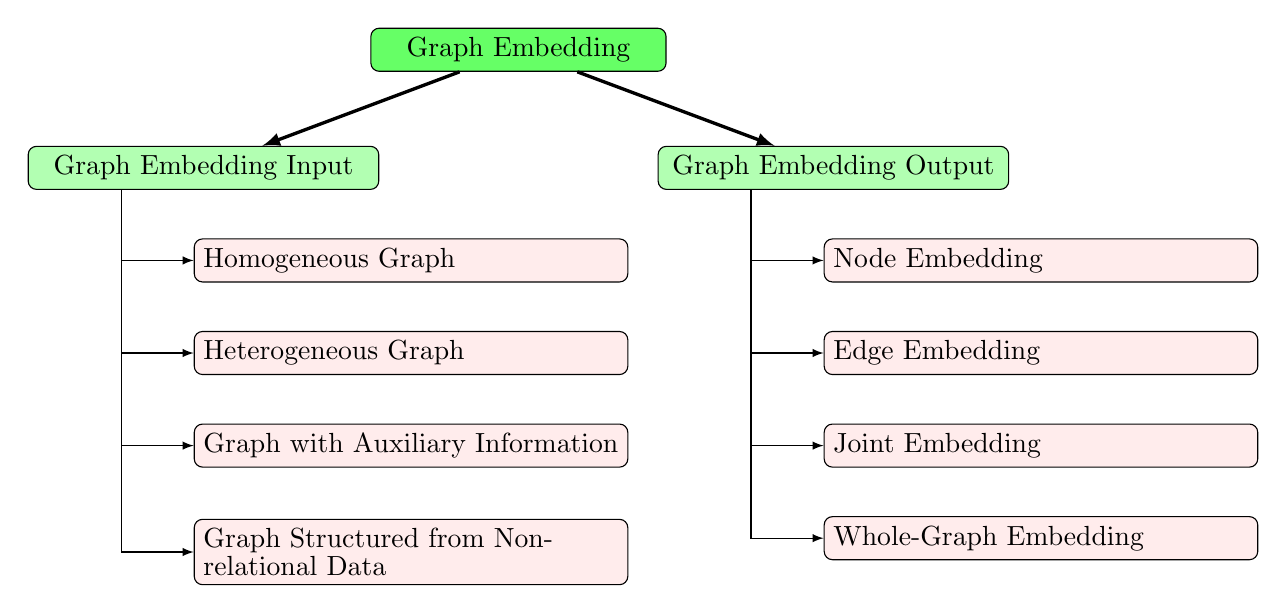
\begin{tikzpicture}[
			rec/.style  = {draw, text width=10cm, rectangle, thin, execute at begin node=\setlength{\baselineskip}{1em}},
			root/.style = {rec, rounded corners=3pt, align=center, fill=green!60, text width=10em},
			level 1/.style={sibling distance=8cm},
			level 2/.style={rec, rounded corners=3pt, fill=green!30,align=center, text width=12em},
			level 3/.style = {rec, rounded corners=3pt, align=left, fill=pink!30, text width=15em, yshift=-20pt},
			edge from parent/.style={->,draw, very thick},
			>=latex]
			
			% root of the the initial tree, level 1
			\node[root] {Graph Embedding}
			child {node[level 2] (c1) {Graph Embedding Input}}
			child {node[level 2] (c2) {Graph Embedding Output}};
			
			% The second level, relatively positioned nodes
			\begin{scope}[every node/.style={level 3}]
				\node [below of = c1, xshift=60pt, yshift=15pt, xshift=15pt] (c11) {Homogeneous Graph};
				\node [below of = c11, yshift=15pt] (c12) {Heterogeneous Graph};
				\node [below of = c12, yshift=15pt] (c13) {Graph with Auxiliary Information};
				\node [below of = c13, yshift=10pt] (c14) {Graph Structured from Non-relational Data};
				
				\node [below of = c2, xshift=60pt, yshift=15pt, xshift=15pt] (c21) {Node Embedding};
				\node [below of = c21, yshift=15pt] (c22) {Edge Embedding};
				\node [below of = c22, yshift=15pt] (c23) {Joint Embedding};
				\node [below of = c23, yshift=15pt] (c24) {Whole-Graph Embedding};
			\end{scope}
			
			% lines from each level 1 node to every one of its "children"
			\foreach \value in {1,...,4}
			\draw[->] (c1.195) |- (c1\value.west);
			
			\foreach \value in {1,...,4}
			\draw[->] (c2.195) |- (c2\value.west);
		\end{tikzpicture}
	}
	\caption{Graph Embedding Techniques}
	\label{fig:graphEmbeddingSettingTree}
\end{figure}




Based on the embedding input, we categorize the surveyed methods in \cite{cai2018comprehensive} as follows: 
Homogeneous Graph, Heterogeneous Graph, Graph with Auxiliary Information, and Graph Constructed from Non-relational Data.

Different types of embedding inputs preserve different information in the embedding space and therefore pose different challenges for the graph embedding problem. 
For example, when embedding a graph with only structural information, the connections between nodes are the primary target to preserve. However, for graphs with node labels or entity attribute information, auxiliary information provides additional context for the graph and can therefore also be considered during the embedding process. Unlike embedding input, which is fixed and provided by the dataset, the embedding output is task-specific.

For instance, the most common embedding output is \textbf{node embedding}, which represents each node as a vector that reflects similarity between nodes. Node embeddings are beneficial for node-related tasks such as node classification, node clustering, etc.

However, in some cases, the tasks may involve more fine-grained graph components such as node pairs, subgraphs, or the entire graph. Therefore, the first challenge of embedding is to determine the appropriate type of embedding output for the application of interest. Four types of embedding outputs are illustrated in \autoref{fig:graphInput}, including: \textbf{Node Embedding} (\ref{fig:nodeEmbedding}), \textbf{Edge Embedding} (\ref{fig:edgeEmbedding}), \textbf{Hybrid Embedding} (\ref{fig:substructureEmbedding}), and \textbf{Whole-Graph Embedding} (\ref{fig:wholeGraphEmbedding}). Different output granularities have distinct criteria and present different challenges. For example, a good node embedding retains similarity with its neighbors in the embedding space. Conversely, a good whole-graph embedding represents the entire graph as a vector that preserves graph-level similarity.


\subsection{Graph Embedding Problem Settings}

While the input is determined by the type of information to be preserved, the output varies depending on the downstream graph mining task. Therefore, we discuss in more detail the embedding methods based on the type of output required by the embedding problem.

\textbf{Node Embedding}
\label{sec:nodeEmbedding}

\begin{figure}[htp]
	\centering
	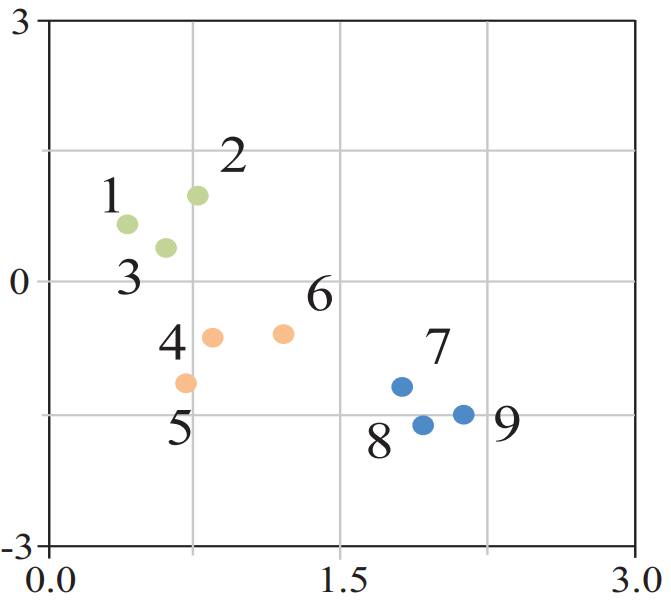
\includegraphics[width=7 cm]{images/graph_emb_2.png}
	\caption{
		Node embedding with each vector representing node features}
	\label{fig:nodeEmbedding}
\end{figure}

Node embedding represents each node as a low-dimensional vector. Nodes that are \textit{close} in the graph have similar vector representations. The difference among graph embedding methods lies in how they define the \textit{closeness} between two nodes. First-order proximity (Definition \ref{def:firstOrderProximity}) and second-order proximity (Definition \ref{def:secondOrderProximity}) are two commonly used metrics to measure pairwise node similarity. Higher-order proximity has also been explored to some extent. For example, capturing k-step (k = 1, 2, 3, ···) neighborhood relationships during embedding is discussed in the study by Cao, Shaosheng \cite{cao2015grarep}.

\textbf{Edge Embedding}
\label{sec:edgeEmbedding}

\begin{figure}[htp]
	\centering
	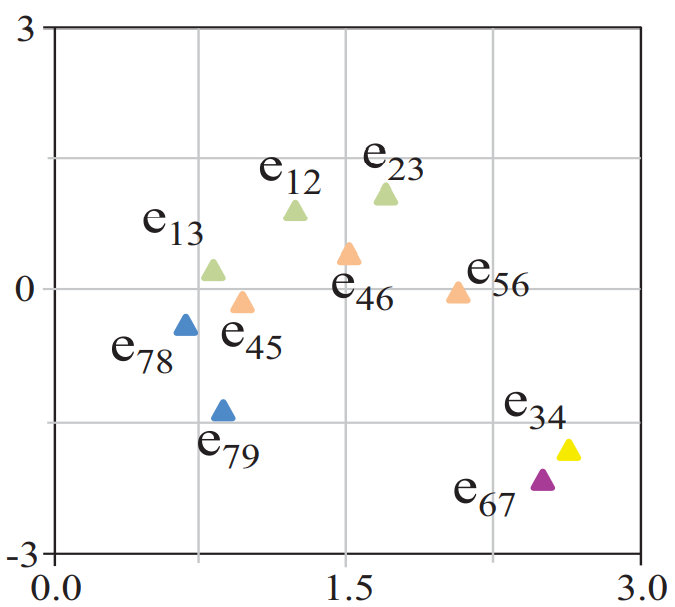
\includegraphics[width=7 cm]{images/graph_emb_3.png}
	\caption{Edge embedding with each vector representing edge features}
	\label{fig:edgeEmbedding}
\end{figure}

In contrast to node embedding, edge embedding aims to represent an edge as a low-dimensional vector. Edge embedding is useful in two cases:

First, in knowledge graph embedding. Each edge is a triple $\langle h, r, t \rangle$ (Definition \ref{def:knowledgeGraph}). The embedding is learned to preserve the relation $r$ between $h$ and $t$ in the embedding space so that a missing entity or relation can be accurately predicted given the other two components in $\langle h, r, t \rangle$.

Second, some methods embed a pair of nodes as a vector to compare it with other node pairs or to predict the existence of a link between the two nodes. Edge embedding benefits graph analyses that involve edges (node pairs), such as link prediction, relation prediction, and knowledge-based entity inference.

\textbf{Hybrid Embedding}

\begin{figure}[htp]
	\centering
	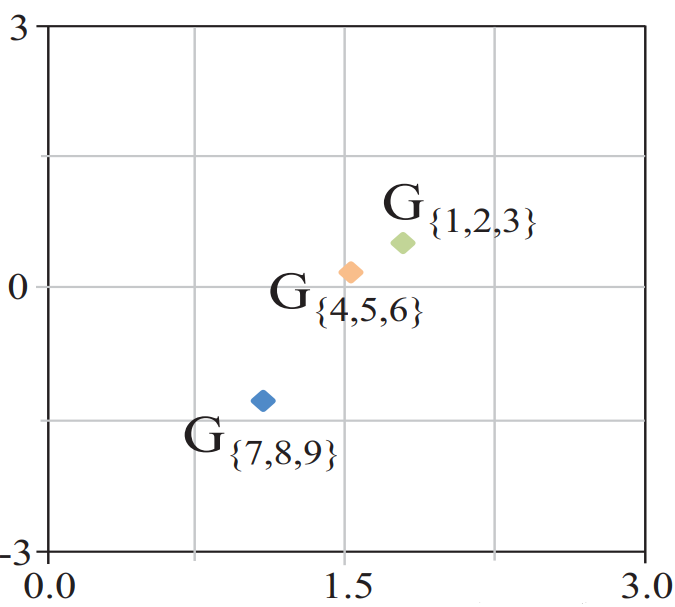
\includegraphics[width=6 cm]{images/graph_emb_4.png}
	\caption{Embedding a graph substructure}
	\label{fig:substructureEmbedding}
\end{figure}

Hybrid embedding refers to embedding combinations of different graph components, e.g., node + edge (i.e., substructure), or node + parts. Substructure or part embeddings can also be derived by aggregating individual node and edge embeddings. However, such \textit{indirect} approaches are not optimized to capture the structure of the graph. Moreover, node and part embeddings can reinforce each other. Node embeddings improve by learning from high-order neighborhood attention, while part embeddings become more accurate due to the collective behavior of their constituent nodes.

\textbf{Whole-Graph Embedding}

\begin{figure}[htp]
	\centering
	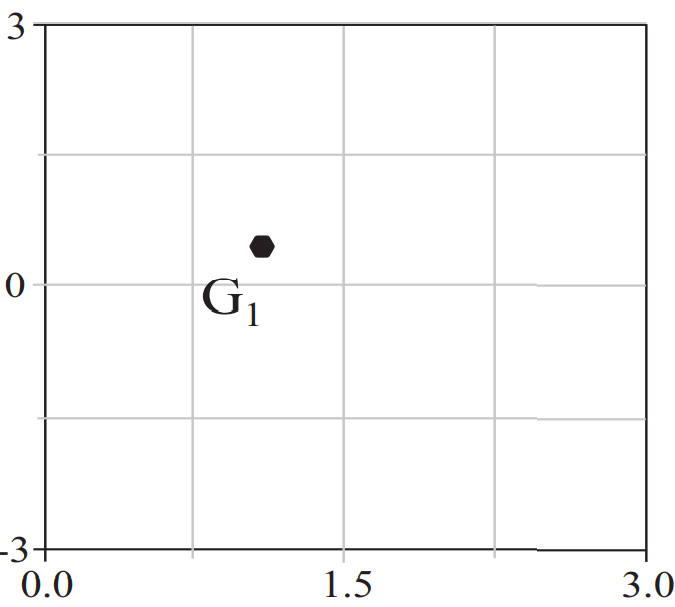
\includegraphics[width=6 cm]{images/graph_emb_5.png}
	\caption{Whole-graph embedding}
	\label{fig:wholeGraphEmbedding}
\end{figure}

Whole-graph embedding is typically used for small graphs such as proteins, molecules, etc. In this case, an entire graph is represented as a vector, and similar graphs are embedded close to each other. Whole-graph embedding is useful for graph classification tasks by providing a simple and effective solution for computing graph similarity. To balance embedding time (efficiency) and information retention (expressiveness), \textbf{hierarchical graph embedding} \cite{mousavi2017hierarchical} introduces a hierarchical embedding framework. It argues that accurate understanding of global graph information requires processing substructures at multiple scales. A graph pyramid is formed where each level is a coarsened graph at a different scale. The graph is embedded at all levels and then concatenated into a single vector. Whole-graph embedding requires collecting features from the entire graph, thus is generally more time-consuming than other settings.


\subsection{Graph Embedding Techniques}

\begin{figure}[htp]
	\centering
	\makebox[\textwidth][l]{
		\hspace{-25mm}
		\resizebox{1.2\textwidth}{!}{%
		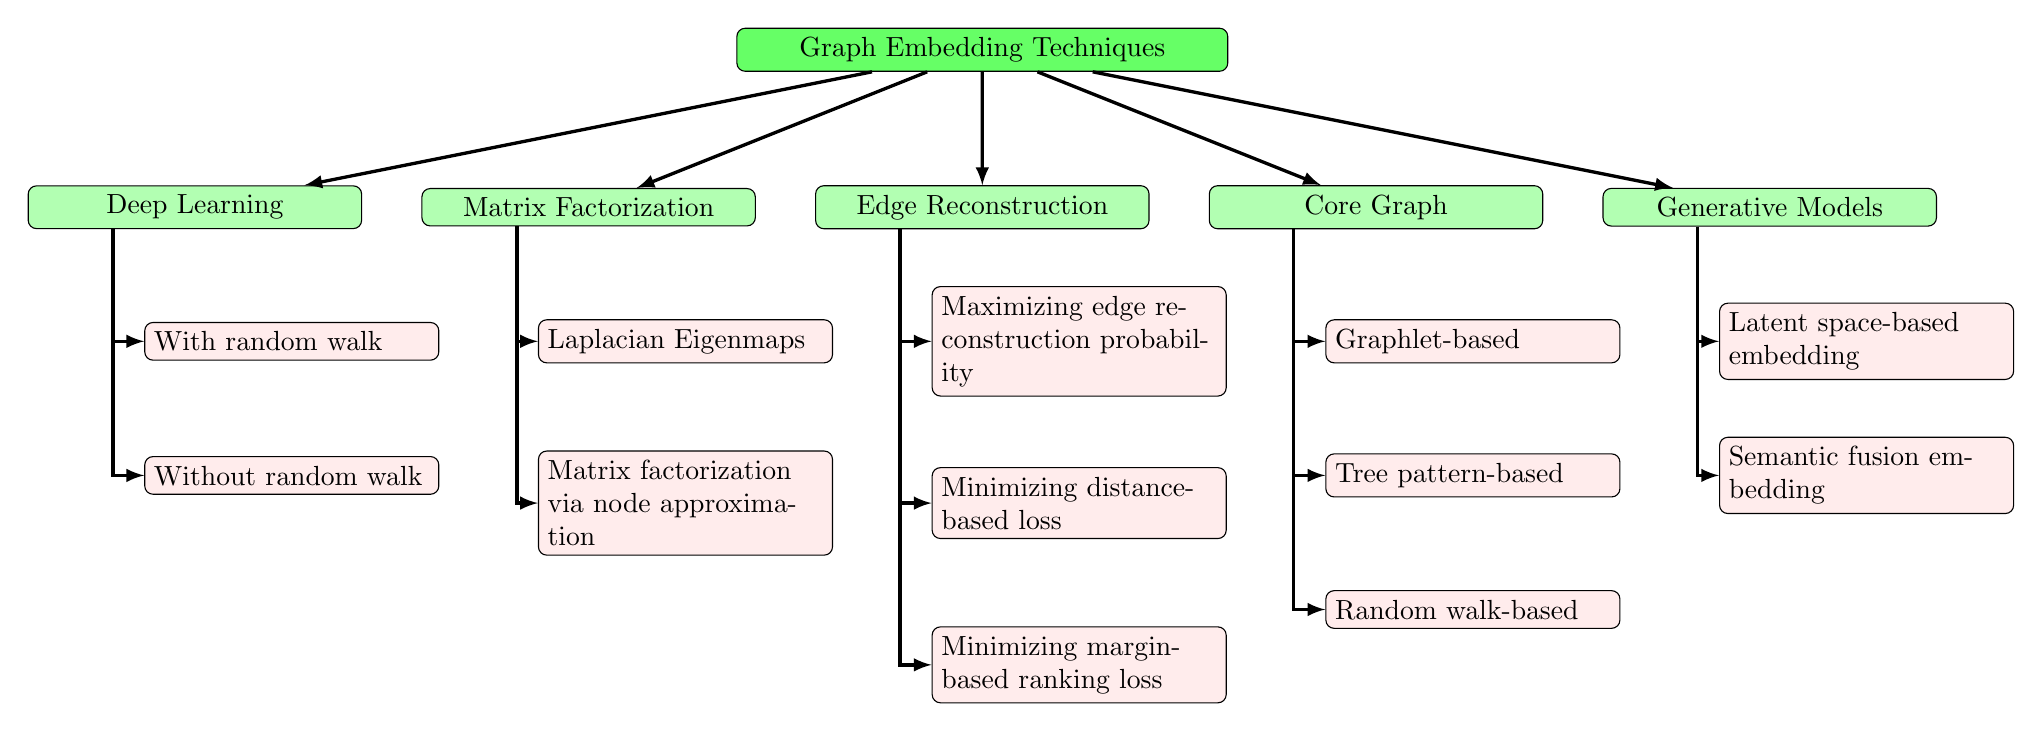
\begin{tikzpicture}[
			rec/.style  = {draw, text width=2.5cm, rectangle, thin, execute at begin node=\setlength{\baselineskip}{1.2em}},
			root/.style = {rec, rounded corners=3pt, align=center, fill=green!60, text width=60mm},
			level 1/.style={sibling distance=50mm, level distance=2cm, text width=60mm},
			level 2/.style={rec, rounded corners=3pt, fill=green!30,align=center, text width=40mm},
			level 3/.style = {rec, align=left, fill=pink!30, text width=35mm, yshift=-20pt, rounded corners=3pt},
			edge from parent/.style={->,draw, very thick},
			>=latex]
			
			\node[root] {Graph Embedding Techniques}
			child {node[level 2] (c1) {Deep Learning}}
			child {node[level 2] (c2) {Matrix Factorization}}
			child {node[level 2] (c3) {Edge Reconstruction}}
			child {node[level 2] (c4) {Core Graph}}
			child {node[level 2] (c5) {Generative Models}};
			
			\begin{scope}[every node/.style={level 3}]
				\node [below of = c1, xshift=35pt] (c11) {With random walk};
				\node [below of = c11] (c12) {Without random walk};
				
				\node [below of = c2, xshift=35pt] (c21) {Laplacian Eigenmaps};
				\node [below of = c21, yshift=-10pt] (c22) {Matrix factorization via node approximation};
				
				\node [below of = c3, xshift=35pt] (c31) {Maximizing edge reconstruction probability};
				\node [below of = c31, yshift=-10pt] (c32) {Minimizing distance-based loss};
				\node [below of = c32, yshift=-10pt] (c33) {Minimizing margin-based ranking loss};
				
				\node [below of = c4, xshift=35pt] (c41) {Graphlet-based};
				\node [below of = c41] (c42) {Tree pattern-based};
				\node [below of = c42] (c43) {Random walk-based};
				
				\node [below of = c5, xshift=35pt] (c51) {Latent space-based embedding};
				\node [below of = c51] (c52) {Semantic fusion embedding};
			\end{scope}
			
			\foreach \value in {1,2}
			\draw[->, very thick] (c1.195) |- (c1\value.west);
			
			\foreach \value in {1, 2}
			\draw[->, very thick] (c2.195) |- (c2\value.west);
			
			\foreach \value in {1,...,3}
			\draw[->, very thick] (c3.195) |- (c3\value.west);
			
			\foreach \value in {1,...,3}
			\draw[->, very thick] (c4.195) |- (c4\value.west);
			
			\foreach \value in {1,...,2}
			\draw[->, very thick] (c5.195) |- (c5\value.west);
		\end{tikzpicture}
	}}
	\caption{Graph Embedding Techniques}
	\label{fig:graphEmbeddingTechniquesTree}
\end{figure}

In this section, we categorize graph embedding methods based on the techniques used. As previously stated, the goal of graph embedding is to represent a graph in a lower-dimensional space while preserving as much of the original graph information as possible. The main differences among embedding techniques lie in how they define which intrinsic graph properties should be preserved. Since the primary focus of our work is on graph embedding methods based on deep learning, we provide only brief overviews of the other method categories.


\textbf{Deep Learning}

In this section, we present in detail the research directions of deep learning techniques, including: using random walks and not using random walks. Deep learning techniques are widely used in graph embedding due to their speed and efficiency in automatically capturing features. Among these deep learning-based methods, three types of input-based graph settings (excluding graphs constructed from non-relational data) and all four output types (as shown in \autoref{fig:graphEmbeddingSettingTree}) can adopt deep learning approaches.

\textit{Deep learning techniques with random walks}

In this category, the second-order proximity (Definition \ref{def:secondOrderProximity}) in the graph is preserved in the embedding space by maximizing the probability of observing a vertex's neighborhood conditioned on its embedding vector. The graph is represented as a set of samples obtained via random walks, and then deep learning methods are applied to ensure the structural properties (i.e., path-based information) are preserved. Representative methods in this group include: DeepWalk \cite{perozzi2014deepwalk}, LINE \cite{tang2015line}, Node2Vec \cite{grover2016node2vec}, Anonymous Walk \cite{ivanov2018anonymous}, NetGAN \cite{bojchevski2018netgan}, etc.

\textit{Deep learning techniques without random walks}

This approach applies multi-layer learning structures effectively and efficiently to transform the graph into a lower-dimensional space. It operates over the entire graph. Several popular methods have been surveyed and presented in \cite{rossi2020knowledge}, as follows:

\begin{itemize}
	\item \textbf{Convolutional Neural Networks (CNNs)}
	
	This model uses multiple convolutional layers: each layer performs convolution on the input data using low-dimensional filters. The result is a feature map, which then passes through a fully connected layer to compute the probability values. For example, \textbf{ConvE} \cite{dettmers2017convolutional}: each entity and relation is represented as a low-dimensional vector ($d$-dimensional). For each triple, it concatenates and reshapes the head $h$ and relation $r$ embeddings into a single input $[h, r]$ with shape $d_m \times d_n$. This is then passed through a convolutional layer with a filter $\omega$ of size $m \times n$, followed by a fully connected layer with weights $W$. The final result is combined with the tail embedding $t$ using a dot product. This architecture can be considered a \textit{multi-class classification} model.
	
	Another popular model is \textbf{ConvKB} \cite{nguyen2017novel}, which is similar to ConvE but concatenates the three embeddings $h$, $r$, and $t$ into a matrix $[h, r, t]$ of shape $d \times 3$. It is then passed through a convolutional layer with $T$ filters of size $1 \times 3$, resulting in a feature map of size $T \times 3$. This is further passed through a fully connected layer with weights $\mathbf{W}$. This architecture can be considered a binary classification model.
	
	\item \textbf{Recurrent Neural Networks (RNNs)}
	
	These models apply one or more recurrent layers to analyze the entire path (a sequence of events/triples) sampled from the training set, instead of treating each event independently. For example, RSN \cite{guo2019learning} notes that traditional RNNs are unsuitable for graphs because each step only takes the relation information without considering the entity embedding from the previous step. Therefore, it fails to clearly model the transitions among entity-relation paths. To address this, they propose RSN (Recurrent Skipping Networks \cite{guo2019learning}): at each step, if the input is a relation, a hidden state is updated to reuse the entity embedding. The output is then dot-multiplied with the target embedding vector.
	
	\item \textbf{Capsule Neural Networks}
	
	Capsule networks group neurons into "capsules" \label{capsule}, where each capsule encodes specific features of the input, such as representing a particular part of an image. One advantage of capsule networks is their ability to capture spatial relationships that are lost in conventional convolution. Each capsule produces feature vectors. For instance, \textbf{CapsE} \cite{vu2019capsule}: each entity and relation is embedded into vectors, similar to ConvKB. It concatenates the embeddings $h$, $r$, and $t$ into a matrix of shape $d \times 3$, then applies $E$ convolutional filters of size $1 \times 3$, resulting in a $d \times E$ matrix. Each $i$-th row encodes distinct features of $h[i]$, $r[i]$, and $t[i]$. This matrix is then fed into a capsule layer, where each capsule (\ref{capsule}) processes a column, thus receiving feature-specific information from the input triple. A second capsule layer is used to produce the final output.
	
	\item \textbf{Graph Attention Networks (GATs)}
	
	This category uses the attention mechanism \cite{vaswani2017attention}, which has achieved notable success in NLP tasks. For each embedding vector, information from neighboring entities is aggregated using attention weights. These are then combined and passed through a fully connected layer with learnable weights to obtain the final embeddings. For example, GAT \cite{velivckovic2017graph} applies multi-head attention to each training triple to generate an embedding vector. This embedding is then transformed via a weight matrix to produce a higher-dimensional vector that aggregates information from neighboring nodes in the original triple. An improved version, KBGAT \cite{nathani2019learning}, incorporates the relation embedding into the attention mechanism. These methods will be discussed in detail in the subsequent sections.
	
	\item \textbf{Other methods}
	
	There are also other approaches, such as autoencoder-based techniques like Structural Deep Network Embedding (SDNE) \cite{wang2016structural}.
\end{itemize}




\textbf{Matrix Factorization}

Matrix factorization-based graph embedding represents the structural characteristics of a graph (e.g., similarity or proximity between vertex pairs) in the form of a matrix and then factorizes this matrix to obtain vertex embeddings. The input for this category of methods is typically high-dimensional non-relational features, and the output is a set of vertex embeddings. There are two matrix factorization-based graph embedding methods: Graph Laplacian Eigenmaps and Node Proximity Matrix Factorization.

\begin{itemize}
	\item \textit{Graph Laplacian Eigenmaps}
	
	This approach preserves graph properties by analyzing similar vertex pairs and heavily penalizes embeddings that place highly similar nodes far apart in the embedding space.
	
	\item \textit{Node Proximity Matrix Factorization}
	
	This approach approximates neighboring nodes in a low-dimensional space using matrix factorization techniques. The objective is to preserve neighborhood information by minimizing the approximation loss.
\end{itemize}

\textbf{Edge Reconstruction}

The edge reconstruction method builds edges based on the vertex embeddings so that the reconstructed graph is as similar as possible to the input graph. This method either maximizes the edge reconstruction probability or minimizes edge reconstruction loss. Additionally, the loss can be distance-based or margin-based ranking loss.

\begin{itemize}
	\item \textit{Maximize Edge Reconstruction Probability}
	
	In this method, a good vertex embedding maximizes the likelihood of generating observed edges in the graph. In other words, a good vertex embedding should allow for reconstructing the original input graph. This is achieved by maximizing the generative probability of all observed edges using vertex embeddings.
	
	\item \textit{Minimize Distance-Based Loss}
	
	In this approach, embeddings of neighboring nodes should be as close as possible to the observed neighboring nodes in the original graph. Specifically, vertex proximity can be measured using their embeddings or heuristically based on observed edges. The difference between these two types of proximity is then minimized to ensure consistent similarity.
	
	\item \textit{Minimize Margin-Based Ranking Loss}
	
	In this approach, the edges in the input graph represent correlations between vertex pairs. Some vertices in the graph are often linked with related vertex sets. This method ensures that embeddings of related nodes are closer together than unrelated ones by minimizing a margin-based ranking loss.
\end{itemize}

\textbf{Graph Kernels}

Graph kernel methods represent the entire graph structure as a vector containing counts of basic substructures extracted from the graph. Subcategories of graph kernel techniques include: graphlets, subtree patterns, and random walk-based methods.

This approach is designed to embed whole graphs, focusing only on global graph features. The input is typically homogeneous graphs or graphs with auxiliary information.

\textbf{Generative Models}

A generative model is defined by specifying a joint distribution over input features and class labels, parameterized by a set of variables. There are two subcategories of generative model-based methods: embedding graphs into latent space and incorporating semantics for embedding. Generative models can be applied to both node and edge embeddings. They are commonly used to embed semantic information, with inputs often being heterogeneous graphs or graphs with auxiliary attributes.

\begin{itemize}
	\item \textit{Embedding Graphs into Latent Semantic Space}
	
	In this group, vertices are embedded into a latent semantic space where the distance between nodes captures the graph structure.
	
	\item \textit{Incorporating Semantics for Embedding}
	
	In this method, each vertex is associated with graph semantics and should be embedded closer to semantically relevant vertices. These semantic relationships can be derived from descriptive nodes via a generative model.
\end{itemize}

\textbf{Summary}: Each graph embedding method has its own strengths and weaknesses, which have been summarized by Cai, Hongyun \cite{cai2018comprehensive} and are presented in \autoref{tab:graphEmbeddingTechCompare}. The \textit{matrix factorization} group learns embeddings by analyzing pairwise global similarities. The \textit{deep learning} group, in contrast, achieves promising results and is suitable for graph embedding because it can learn complex representations from complex graph structures.

\newcolumntype{L}{>{\arraybackslash}m{0.25\textwidth}}
\newcolumntype{M}{>{\arraybackslash}m{0.2\textwidth}}
\begingroup
\normalsize
\setlength{\tabcolsep}{8pt}
\begin{longtable}{|p{0.2\textwidth}|p{0.22\textwidth}|L|p{0.22\textwidth}|}
	\caption{Comparison of Advantages and Disadvantages of Graph Embedding Techniques} \label{tab:graphEmbeddingTechCompare} \\
	\hline
	Method & Subcategory & Advantages & Disadvantages \\
	\hline \hline
	\endfirsthead
	
	%	\multicolumn{4}{c}%
	%	{{\bfseries \tablename\ \thetable{} -- continued from previous page}} \\
	\hline
	Method & Subcategory & Advantages & Disadvantages \\
	\hline \hline
	\endhead
	
	%	\hline \multicolumn{4}{|r|}{{Continued on next page}} \\ \hline
	\endfoot
	
	\hline
	\endlastfoot
	
	Matrix Factorization & Graph Laplacian Eigenmaps & \multirow{3}{=}{Considers global neighborhood structure} &
	\multirow{2}{=}{Requires large computation time and space} \\ \cline{2-2}
	& Node Proximity Matrix Factorization & & \\
	\hline
	\multirow{3}{=}{Edge Reconstruction} & Maximize edge reconstruction probability & \multirow{3}{=}{Relatively efficient training} & \multirow{3}{=}{Only optimizes local information, e.g., first-order neighbors or ranked node pairs} \\ \cline{2-2}
	& Minimize distance-based loss & & \\ \cline{2-2}
	& Minimize margin-based ranking loss & & \\ \hline
	\multirow{3}{=}{Graph Kernels} & Based on graphlet & \multirow{3}{=}{Efficient, considers only desired primitive structures} & \multirow{3}{=}{Substructures are not independent. Embedding dimensionality increases exponentially} \\ \cline{2-2}
	& Based on subtree patterns & & \\ \cline{2-2}
	& Based on random walk & & \\ \hline
	
	Generative Model & Embedding into latent space & Embedding is interpretable & Difficult to tune distribution selection \\ \cline{2-3}
	
	& Incorporate semantics & Leverages multiple information sources & Requires a large amount of naturally labeled data\\
	\hline
	
	Deep Learning & With random walk & \multirow{2}{=}{Efficient and fast. No need for manual feature extraction} & Considers only local path content. Difficult to find optimal sampling strategy \\ \cline{2-2} \cline{4-4} 
	& Without random walk & & High computational cost \\ \hline
\end{longtable}
\endgroup



%\newcolumntype{L}{>{\arraybackslash}m{5cm}}
%\begin{table}[htbp]
%	\begin{center}
%		\caption{Bảng so sánh ưu và nhược điểm của kỹ thuật nhúng đồ thị}
%		\label{tab:graphEmbeddingTechCompare2}
%		\resizebox{\textwidth}{!}{
%			\begin{tabular}{|p{2cm}|p{8cm}|L|p{8cm}|}
%				\hline
%				Phương pháp & Danh mục con & Ưu điểm & Nhược điểm \\
%				\hline \hline
%				Phân rã ma trận & Đồ thị toán tử Laplace Eigenmap & \multirow{3}{5cm}{Xem xét toàn cục các đỉnh lân cận}&
%				\multirow{2}{8cm}{Sử dụng không gian và thời gian tính toán lớn }\\
%				\cline{2-2}
%				& Phân rã ma trận bằng xấp xỉ đỉnh & & \\
%				\hline
%				\multirow{3}{2cm}{Tái cấu trúc cạnh} & Cực đại hóa xác suất tái cấu trúc cạnh & \multirow{3}{5cm}{Huấn luyện tương đối hiệu quả} & \multirow{3}{8cm}{Tối ưu chỉ sử dụng thông tin cục bộ. Ví dụ như các cạnh (hàng xóm 1 nước) hoặc cặp đỉnh xếp hạng } \\ \cline{2-2}
%				& Tối thiểu hóa mất mát dựa trên khoảng cách & & \\ \cline{2-2}
%				& Tối thiểu hóa xếp hạng mất mát dựa trên lề & & \\ \hline
%				\multirow{3}{2cm}{Đồ thị lõi} & Dựa trên graphlet & \multirow{3}{5cm}{Hiệu quả, chỉ tính những nhánh cấu trúc đơn vị mong muốn} & \multirow{3}{8cm}{Nhánh cấu trúc thì không độc lập. Số chiều nhúng tăng lên theo hàm mũ} \\ \cline{2-2}
%				& Dựa trên mẫu nhánh cây   & & \\ \cline{2-2}
%				& Dựa trên bước nhảy ngẫu nhiên & & \\ \hline
%				
%				Mô hình sinh & Nhúng đồ thị dựa trên không gian ẩn & Phép nhúng có thể giải thích được & Khó điều chỉnh lựa chọn phân bố \\ \cline{2-3}
%				
%				& Nhúng kết hợp ngữ nghĩa & Tận dụng nhiều thông tin nguồn & Yêu cầu một lượng lớn dữ liệu huấn luyện một cách tự nhiên\\
%				\hline
%				
%				Học sâu & Sử dụng bước ngẫu nhiên & \multirow{2}{5cm}{Hiệu quả và nhanh chóng Không phải trích đặc trưng} & Chỉ xem xét đến nội dung cục bộ trong một đường đi. Khó để tìm kiếm chiến lược lấy mẫu tối ưu \\ \cline{2-2} \cline{4-4} 
%				& Không sử dụng bước ngẫu nhiên &  & Chi phí tính toán cao \\ \hline
%			\end{tabular}
%		}
%	\end{center}
%\end{table}
	

Graph embedding methods based on random walk in deep learning have lower computational cost compared to those using full deep learning models. Traditional methods often treat graphs as grids; however, this does not reflect the true nature of graphs. In the \textit{edge reconstruction} group, the objective function is optimized based on observed edges or by ranking triplets. While this approach is more efficient, the resulting embedding vectors do not account for the global structure of the graph. The \textit{graph kernel} methods transform graphs into vectors, enabling graph-level tasks such as graph classification. Therefore, they are only effective when the desired primitive structures in a graph can be enumerated. The \textit{generative model} group naturally integrates information from multiple sources into a unified model. Embedding a graph into a latent semantic space produces interpretable embedding vectors using semantics. However, assuming the modeling of observations using specific distributions can be difficult to justify. Moreover, generative approaches require a large amount of training data to estimate a model that fits the data well. Hence, they may perform poorly on small graphs or when only a few graphs are available.

Among these methods, deep learning-based graph embedding allows learning complex representations and has shown the most promising results. Graph attention networks (GATs), which are based on attention mechanisms, aggregate the information of an entity using attention weights from its neighbors relative to the central entity. We believe this research direction is aligned with studies on the relationship between attention and memory \cite{memoryandattention:2020}, where the distribution of attention determines the weight or importance of one entity relative to another. Likewise, the embedding vector representing an entity is influenced by the attention or importance of its neighboring embeddings. Therefore, this is the approach we selected among the existing graph embedding methods.

\section{Multi-head Attention Mechanism}

In 2014, the multi-head attention mechanism was introduced by Bahdanau, Dzmitry \cite{bahdanau2014neural}, but it only gained widespread popularity in 2017 through the Transformer model by Vaswani, Ashish \cite{vaswani2017attention}. The attention mechanism is an effective method to indicate the importance of a word with respect to other words in a sentence, and it has been shown to be a generalization of any convolution operation as reported by Cordonnier, Jean-Baptiste \cite{cordonnier2019relationship}. To understand how multi-head attention is applied to graphs, in this section we will detail the mechanism so we can better understand how it is used in link prediction tasks within knowledge graphs.

\subsection{Attention Mechanism}
\label{sec:attentionMechanism}

The input of the attention mechanism consists of two embedding matrices $\mathbf{X} = \Big\{\overrightarrow{x_1}, \overrightarrow{x_2}, ...,  \overrightarrow{x_{N_x}}\Big\}$ and $\mathbf{Y} = \Big\{\overrightarrow{y_1}, \overrightarrow{y_2}, ...,  \overrightarrow{y_{N_y}}\Big\}$, where each row $i^{\text{th}}$ or $j^{\text{th}}$ in matrix $\mathbf{X}$ or $\mathbf{Y}$ is an embedding vector $\overrightarrow{x_i} \in \mathbb{R}^{1 \times D_{\text{in}}}$, $\overrightarrow{y_j} \in \mathbb{R}^{1 \times D_{\text{in}}}$.

The attention mechanism transforms input vectors of $D_{\text{in}}$ dimensions into output vectors of $D_{\text{attention}}$ dimensions to represent the importance of each of the $N_x$ elements $x$ with respect to all $N_y$ elements $y$. Given $\mathbf{X} \in \mathbb{R}^{N_x \times D_\text{in}}$ and $\mathbf{Y} \in \mathbb{R}^{N_y \times D_\text{in}}$ as input embedding matrices, and $\mathbf{H} \in \mathbb{R}^{N_x \times D_\text{attention}}$ as the output embedding matrix, the attention mechanism introduced by Vaswani et al. \cite{vaswani2017attention} is defined as follows:

\begin{equation}
	\label{attention}
	\mathbf{H} = \text{Attention}(\mathbf{Q}, \mathbf{K}, \mathbf{V}) = \text{softmax}\Big(\frac{\mathbf{Q}\mathbf{K}^T}{\sqrt{d_k}}\Big) \mathbf{V}
\end{equation}

where $\mathbf{Q} = \mathbf{X}\mathbf{W}_Q, \mathbf{K} = \mathbf{Y} \mathbf{W}_K, \mathbf{V} = \mathbf{Y} \mathbf{W}_V$.

The weight matrices 
$\mathbf{W}_Q \in \mathbb{R}^{D_{\text{in}} \times D_{k}}$, 
$\mathbf{W}_K \in \mathbb{R}^{D_{\text{in}} \times D_{k}}$, and 
$\mathbf{W}_V \in \mathbb{R}^{D_{\text{in}} \times D_{\text{attention}}}$ 
are used to parameterize the transformation from input embedding vectors of dimension $D_{\text{in}}$ into output embedding vectors of dimension $D_k$ or $D_{\text{attention}}$. The term $\mathbf{Q}\mathbf{K}^T$ represents the dot product between each vector $x$ and all vectors $y$. Dividing by $\sqrt{d_k}$ normalizes the result with respect to the vector dimension $k$. The result is then passed through the \textit{softmax} function to enable comparison of attention scores across different pairs. We can interpret $\text{softmax}\Big(\frac{\mathbf{Q}\mathbf{K}^T}{\sqrt{d_k}}\Big)$ as the \textit{attention coefficients}, indicating the importance of each $y$ with respect to each $x$. Finally, this is multiplied with the value matrix $\mathbf{V}$ to produce the final output embedding of dimension $D_{\text{attention}}$.

If $\mathbf{X} = \mathbf{Y}$, we are computing the importance of each element with respect to other elements in the same input matrix, which is referred to as the self-attention mechanism.


\subsection{Multi-Head Attention}

The multi-head attention mechanism is a way of combining multiple attention layers to stabilize the learning process. Similar to the standard attention mechanism above, the multi-head attention mechanism transforms the initial $N_x$ embedding vectors of dimension $D_{\text{in}}$ into output embedding vectors of dimension $D_{\text{multi-head}}$, aggregating information from various other nodes to provide greater stability during training. Multi-head attention stacks $N_{\text{head}}$ attention output matrices $\mathbf{H}$, and then applies a weight matrix to transform the original embedding matrix $\mathbf{X} \in \mathbb{R}^{N_x \times D_\text{in}}$ into a new embedding matrix $\mathbf{X}' \in \mathbb{R}^{N_x \times D_{\text{multi-head}}}$ using the following formula:

\begin{equation}
	\label{headAttention}
	\begin{split}
		\mathbf{X}'& =\left(\bigparallel_{h=1}^{N_{\text{head}}}\mathbf{H}^{(h)}\right)\mathbf{W}^{O} \\
		& = \left(\bigparallel_{h=1}^{N_{\text{head}}} \text{Attention}(\mathbf{X} \mathbf{W}_Q^{(h)}, \mathbf{Y} \mathbf{W}_K^{(h)}, \mathbf{Y} \mathbf{W}_V^{(h)}) \right)\mathbf{W}^{O}
	\end{split}
\end{equation}

Here, the weight matrices $\mathbf{W}_Q^{(h)}$, $\mathbf{W}_K^{(h)} \in \mathbb{R}^{D_{\text{in}} \times D_{k}}$, and $\mathbf{W}_V^{(h)} \in \mathbb{R}^{D_{\text{in}} \times D_{\text{attention}}}$ correspond to each individual attention head $h \in [N_{\text{head}}]$. The output projection matrix $\mathbf{W}^{O} \in \mathbb{R}^{N_{\text{head}} D_{\text{attention}} \times D_{\text{multi-head}}}$ parameterizes the transformation of the concatenated output heads into the final output embedding matrix.

At this point, we have presented the attention mechanism for computing attention scores and aggregating embedding information from neighboring vectors. In the next section, we will describe how this attention mechanism is applied to knowledge graphs.

%\textbf{Lớp cộng tác đa đỉnh chú ý}

%\cite{weng2018attention}

\section{Graph Attention Network}
\label{sec:GAT}

\begin{figure}[htp]
	\centering
	\resizebox{\textwidth}{!}{%
		\begin{tikzpicture}[
			entityStyle/.style={draw, color=white, thin, align=center, circle, text width=20mm},
			us/.style = {entityStyle, fill=amber},
			entity/.style={entityStyle, fill=azure},
			arrowStyle/.style={-latex', >=stealth },
			entityId/.style={draw, color=white,  thin, align=center, circle},]
			
			\node[us] (us) {\textbf{U.S}};
			
			\begin{scope}[every node/.style={entity}]
				\node[above left=2cm of us, xshift=-20mm] (c1) {\textbf{Donald Trump}};
				\node[above right=2cm of us, xshift=1cm] (c2) {\textbf{Jeff Bezos}};
				\node[below left=2cm of us, xshift=-20mm] (c3) {\textbf{New York}};
				\node[below right=2cm of us, xshift=1cm] (c4) {\textbf{Tesla Inc.}};
				
				\node[below left=3cm of c1, yshift=25mm, xshift=-15mm] (c1x) {\textbf{Melania Trump}};
				\node[above left=3cm of c3, yshift=-25mm, xshift=-15mm] (c3x) {\textbf{Tom Cruise}};
				
				%\node[left=1cm of c1x, yshift=25mm, xshift=-15mm] (c8) {\textbf{Thanh}};
			\end{scope}
			
			%\draw[->, line width=0.8mm, azure] (c8) -> (c1x);
			%\path[arrowStyle] (c8)--node[rotate=-31, yshift=4mm]{friend\_of} %node[rotate=-31, yshift=-3mm]{} (c1x);
			
			\foreach \value in {1,...,4}
			\draw[->, line width=0.8mm, azure] (c\value) -> (us);
			\foreach \value in {1,3}
			\draw[->, line width=0.8mm, azure] (c\value x) -> (c\value);
			
			\foreach \value in {1,3}
			\draw[->, line width=0.8mm, azure!60, dash pattern=on 3mm off 1mm, postaction={decorate}] (c\value x) -> (us);
			
			\path[arrowStyle] (c1)--node[rotate=-31, yshift=4mm]{president\_of} node[rotate=-31, yshift=-3mm]{$\alpha_{i4}$} (us);
			
			\path[arrowStyle] (c3)--node[rotate=30, yshift=4mm]{state\_of} node[rotate=30, yshift=-4mm]{$\alpha_{i3}$} (us);
			
			\path[arrowStyle] (c2)--node[rotate=41, yshift=4mm]{richest\_of} node[rotate=41, yshift=-4mm]{$\alpha_{i1}$} (us);
			
			\path[arrowStyle] (c4)--node[rotate=-41, yshift=4mm]{founded\_in} node[rotate=-41, yshift=-4mm]{$\alpha_{i2}$} (us);
			
			\path[arrowStyle] (c1x)--node[rotate=15, yshift=4mm]{wife\_of} (c1);
			\path[arrowStyle] (c3x)--node[rotate=-15, yshift=4mm]{born\_in} (c3);
			
			\path[arrowStyle] (c1x)--node[rotate=-8, yshift=4mm]{\textbf{first\_lady}} node[rotate=-8, yshift=-3mm]{$\alpha_{i5}$} (us);
			\path[arrowStyle] (c3x)--node[rotate=8, yshift=4mm]{\textbf{native\_of}} node[rotate=8, yshift=-3mm]{$\alpha_{i6}$} (us);
			
			%%%%%%%%%%%
			\node[entityId][fill=amber][right=11cm of us] (country) {$e_3$};
			\path[arrowStyle] (us)--node[yshift=2mm]{\LARGE $\rightarrow$} (country);
			
			\begin{scope}[every node/.style={entityId, fill=azure}]
				\node[above left=1cm of country, xshift=-5mm] (c1s) {$e_2$};
				\node[above right=1cm of country, xshift=5mm] (c2s) {$e_4$};
				\node[below left=1cm of country, xshift=-5mm] (c3s) {$e_6$};
				\node[below right=1cm of country, xshift=5mm] (c4s) {$e_7$};
				
				\node[below left=1.5cm of c1s, yshift=15mm, xshift=-5mm] (c1xs) {$e_1$};
				\node[above left=1.5cm of c3s, yshift=-15mm, xshift=-5mm] (c3xs) {$e_5$};
			\end{scope}
			\foreach \value in {1,...,4}
			\draw[->, line width=0.8mm, azure] (c\value s) -> (country);
			\foreach \value in {1,3}
			\draw[->, line width=0.8mm, azure] (c\value xs) -> (c\value s);
			
			\foreach \value in {1,3}
			\draw[->, line width=0.8mm, azure!60, dash pattern=on 3mm off 1mm, postaction={decorate}] (c\value xs) -> (country);
			
			\path[arrowStyle] (c1s)--node[rotate=-31, yshift=2mm]{$r_2$} (country);
			
			\path[arrowStyle] (c3s)--node[rotate=30, yshift=2mm]{$r_5$} (country);
			
			\path[arrowStyle] (c2s)--node[rotate=41, yshift=2mm]{$r_3$} (country);
			
			\path[arrowStyle] (c4s)--node[rotate=-41, yshift=2mm]{$r_6$} (country);
			
			\path[arrowStyle] (c1xs)--node[rotate=15, yshift=2mm]{$r_1$} (c1s);
			\path[arrowStyle] (c3xs)--node[rotate=-15, yshift=2mm]{$r_4$} (c3s);
			
			\path[arrowStyle] (c1xs)--node[rotate=-8, yshift=2mm]{$r_7$} (country);
			\path[arrowStyle] (c3xs)--node[rotate=8, yshift=2mm]{$r_8$} (country);
		\end{tikzpicture}
	}
	\caption{Knowledge graph and normalized attention coefficients of the entity}
	\label{fig:graphExample}
\end{figure}

With the success of the \textit{multi-head attention mechanism} in natural language processing, it has also been studied for applications in image processing models \cite{ramachandran2019stand}. Consequently, the multi-head attention mechanism has been explored for replacing convolutional operations in knowledge graph embedding models, such as Graph Convolutional Networks (GCNs \cite{kipf2016semi}). In this section, we present in detail how the attention mechanism from \ref{sec:attentionMechanism} is applied to graph embedding via the Graph Attention Network (GAT \cite{velivckovic2017graph}) method.

The input to the \textit{graph attention network} model is a set of embedding vectors, randomly initialized from a normal distribution, representing features of each entity: $\mathbf{E} = \Big\{\overrightarrow{e_1}, \overrightarrow{e_2}, ...,  \overrightarrow{e_{N_e}}\Big\}$. The objective of the model is to transform this into a new output embedding matrix $\mathbf{E}'' = \Big\{\overrightarrow{e''_1}, \overrightarrow{e''_2}, ...,  \overrightarrow{e''_{N_e}}\Big\}$ capable of aggregating embedding information from neighboring entities. Here, $\mathbf{E} \in \mathbb{R}^{N_e \times D_{\text{in}}}$ and $\mathbf{E}'' \in \mathbb{R}^{N_e \times D''}$ denote the input and output embedding matrices for the entity set, respectively. $N_e$ is the number of entities, and $D_{\text{in}}$, $D''$ are the dimensions of the input and output embeddings.

Similar to the multi-head attention mechanism introduced in \ref{sec:attentionMechanism}, the application of this mechanism to a knowledge graph follows the same logic as the \textit{self-attention mechanism}, in which each node attends to all other nodes in the graph. However, computing attention scores between every pair of nodes in a graph is not meaningful if no relationship exists between them, and it would incur significant computational overhead. Therefore, the model applies a technique known as \textit{masked attention}, in which all attention scores corresponding to unrelated nodes in the graph are ignored. These relevant connections are precisely defined as the first-order proximity (Definition \ref{def:firstOrderProximity}) of a node in the graph. Thus, in this context, we let $\mathbf{X} = \mathbf{Y} = \mathbf{E}$ (as in \ref{sec:attentionMechanism}), and the attention coefficient in the masked attention mechanism represents the importance of a neighboring node $j \in \mathcal{N}_{i}$ to the central node $i$, where $\mathcal{N}_{i}$ is the set of all first-order neighbors of node $i$ (including $i$ itself).




The application of the multi-head attention mechanism (\textit{multi-head attention}) in \ref{headAttention} to graphs is described as follows:

\begin{equation}
	\label{maskAttention}
	\centering
	{e_{ij}}={f_{\text{mask attention}}(\mathbf{W} \overrightarrow{e_i}, \mathbf{W} \overrightarrow{e_j})}
\end{equation}

where $e_{ij}$ denotes the multi-head attention coefficient of an edge $(e_i, e_j)$ with respect to the central entity $e_i$ in the knowledge graph $\mathcal{G}_{\text{know}}$. $\mathbf{W}$ is a weight matrix that parameterizes the linear transformation. $f_{\text{mask attention}}$ is the function applying the attention mechanism.

In the GAT model, each entity vector embedding $\overrightarrow{e_i}$ undergoes two transformation stages. The entire model consists of two transformation steps, each applying the multi-head attention mechanism as follows:

\begin{equation}
	\label{gatProcess}
	\overrightarrow{e_i} \xrightarrow{f_{\text{mask attention}}^{(1)}} \overrightarrow{e'_i} \xrightarrow{f_{\text{mask attention}}^{(2)}} \overrightarrow{e''_i}
\end{equation}

In the first multi-head attention step ($f_{\text{mask attention}}^{(1)}$), the model aggregates information from neighboring entities and stacks them to produce vector $\overrightarrow{e'_i}$, where $\overrightarrow{e'_i} \in \mathbb{R}^{1 \times D'}$. In the second step ($f_{\text{mask attention}}^{(2)}$), the multi-head attention layer is no longer sensitive to self-attention; therefore, the output is computed as an \textit{average} instead of concatenating attention heads. The vector $\overrightarrow{e'_i}$ is then treated as the input embedding to be transformed into the final output embedding vector $\overrightarrow{e''_i}$, with $\overrightarrow{e''_i} \in \mathbb{R}^{1 \times D''}$.

First, similar to the attention mechanism in \ref{attention}, each embedding vector is multiplied by a weight matrix $\mathbf{W}_1 \in \mathbb{R}^{D_k \times D_{\text{in}}}$ to parameterize the linear transformation from $D_{\text{in}}$ input dimensions to $D_k$ higher-level feature dimensions:

\begin{equation}
	\overrightarrow{h_i} = \mathbf{W}_{1} \overrightarrow{e_i}
\end{equation}

where $\overrightarrow{e_i} \in \mathbb{R}^{D_{\text{in}} \times 1}
\xrightarrow{} \overrightarrow{h_i} \in \mathbb{R}^{D_k \times 1}$


Next, we concatenate each pair of linearly transformed entity embedding vectors to compute the attention coefficients. The attention coefficient $e_{ij}$ reflects the importance of the edge feature $(e_i, e_j)$ with respect to the central entity $e_i$, or in other words, the importance of a neighboring entity $e_j$ that is connected to $e_i$. We apply the $\text{LeakyReLU}$ function to extract the absolute value of the attention coefficient. Each attention coefficient $e_{ij}$ is computed using the following equation:

\begin{equation}
	e_{ij} = \Big( \text{LeakyReLU} \Big( \overrightarrow{\mathbf{W}_{2}}^{T} [\overrightarrow{h_i} || \overrightarrow{h_j}]\Big) \Big)
\end{equation}

where ${.}^{T}$ denotes the transpose operation and $||$ represents concatenation. This is similar to \ref{attention}, however instead of using a dot product, we use a \textit{shared attentional mechanism} $\overrightarrow{\mathbf{W}_2}$: $\mathbb{R}^{D_k} \times \mathbb{R}^{D_k} \rightarrow \mathbb{R}$ to compute the attention scores. As mentioned in \ref{maskAttention}, we perform self-attention between all nodes using the masked attention mechanism to discard all irrelevant structural information.

To enable meaningful comparison between the attention coefficients of neighboring entities, a \textit{softmax} function is applied to normalize the coefficients over all neighbors $e_j$ that are connected to the central entity $e_i$: $\alpha_{ij} = \text{softmax}_j(e_{ij})$. Combining all of this, we obtain the final normalized attention coefficient of each neighbor with respect to the central entity as follows:

\begin{equation}
	\label{attentionCoeff}
	\alpha_{ij} = \frac{
		\text{exp} \Big( \text{LeakyReLU} \Big( \overrightarrow{\mathbf{W}_2}^{T} [ \overrightarrow{h_i} || \overrightarrow{h_j}]\Big) \Big))
	}
	{
		\sum_{k \in \mathcal{N}_i}
		\text{exp} \Big( \text{LeakyReLU} \Big( \overrightarrow{\mathbf{W}_2}^{T} [\overrightarrow{h_i} || \overrightarrow{h_k}]\Big) \Big))
	}
\end{equation}





At this stage, the GAT model operates similarly to GCN \cite{kipf2016semi}, where the embedding vectors from neighboring nodes are aggregated and scaled by their corresponding normalized attention coefficients:

\begin{equation}
	\label{scaleAttentionCoef}
	\centering
	{\overrightarrow{e'_i}}={\sigma\left(\sum_{j\in \mathcal{N}_i} {\alpha_{ij} \overrightarrow{h_j} }\right)}
\end{equation}

Similar to the multi-head attention layer, we concatenate $N_{\text{head}}$ attention heads to stabilize the training process in the first step ($f_{\text{mask attention}}^{(1)}$ \ref{gatProcess}) of the model:

\begin{equation}
	\label{multiHeadAttention}
	{\overrightarrow{e'_i}}={\bigparallel_{h=1}^{N_{\text{head}}}\sigma\left(\sum_{j\in \mathcal{N}_i}\alpha_{ij}^{h} \mathbf{W}^{h} \overrightarrow{h_{j}} \right)}
\end{equation}

where $\sigma$ is any non-linear activation function, and $\alpha_{ij}^h$ is the normalized attention coefficient for edge $(e_i, e_j)$ computed from the $h^{th}$ attention head. Similar to equation \ref{attention}, $\mathbf{W}^h$ is the weight matrix used for linear transformation of the input embedding vector, with each $\mathbf{W}^h$ corresponding to a different attention head. The resulting new embedding vector $\overrightarrow{e'_i} \in \mathbb{R}^{1 \times D'}$, where $D' = N_{\text{head}} D_{\text{k}}$, is then used as the input for the next attention layer. However, in the second step ($f_{\text{mask attention}}^{(2)}$ \ref{gatProcess}), the multi-head attention outputs are averaged instead of concatenated, as shown below:

\begin{equation}
	\label{multiHeadConcat}
	{\overrightarrow{e''_i}}={\sigma\left(\frac{1}{N_{\text{head}}} \sum_{h=1}^{N_{\text{head}}}\sum_{j\in \mathcal{N}_i}\alpha_{ij}^{h} \mathbf{W}^{h} \overrightarrow{e'_{j}} \right)}
\end{equation}



\textbf{Summary}: Up to this point, we have presented how the attention mechanism aggregates a knowledge graph entity embedding vector from its neighboring embeddings and concatenates them to produce the final embedding. In the next section, we will present our complete embedding model based on the KBGAT model proposed by Nathani, Deepak\cite{nathani2019learning}.

\section{KBGAT Model}

In a knowledge graph, a single entity cannot fully represent an edge, as the entity can play multiple roles depending on the type of relation. For example, in \autoref{fig:graphExample}, Donald Trump serves both as a president and as a husband. To address this issue, the knowledge graph attention-based embedding model — KBGAT (graph attention based embeddings \cite{nathani2019learning}) — improves upon the GAT model by incorporating additional information from \textit{relations and neighboring node features} into the attention mechanism. In this section, we will detail the KBGAT model. The structure of KBGAT follows an encoder-decoder framework, where the encoder is implemented using the Graph Attention Network (GAT), and the decoder uses the ConvKB model for prediction. The steps of the KBGAT model are illustrated in \ref{eq:KBGATProcess}.

\begin{equation}
	\label{eq:KBGATProcess}
	entities \xrightarrow{\text{Embedding}^{\ref{sec:initTransE}}} \overrightarrow{e_{\text{TransE}}} \xrightarrow{\text{Embedding} ^{\ref{sec:encodeKBGAT}}} \overrightarrow{e_{\text{KBGAT}}} \xrightarrow{\text{ConvKB}^{\ref{sec:predictionConvKB}}} e_{\text{prob}}
\end{equation}

First, the embedding vectors of each entity are initialized using the TransE model to capture the spatial characteristics among nodes and obtain the initial embeddings. These embeddings are then further trained using an encoder model to capture neighborhood features, resulting in updated embeddings. Finally, these embeddings are passed through a prediction layer using the ConvKB model. All equations presented here are based on those in the work of Nathani, Deepak\cite{nathani2019learning}.




\subsection{Embedding Initialization}
\label{sec:initTransE}

\begin{figure}[htp]
	\centering
	\begin{tikzpicture}[
		arrow/.style={->,thick},
		vector/.style={arrow, ultra thick},
		dashLine/.style={->, thin, dash pattern=on 1mm off 0.5mm},
		formal/.style={font=\sffamily}]
		\coordinate (root) at (0,0);
		\coordinate [formal, label=above left:$\overrightarrow{\text{relation}}$] (c1) at (-1.5, 3);
		\coordinate [formal, label=above:$\overrightarrow{\text{tail}_{\text{invalid}}}$] (c2) at (3.5, 5);
		\coordinate [formal, label=right:$\overrightarrow{\text{tail}_{\text{valid}}}$] (c3) at (3.5, 4);
		\coordinate [formal, label=above right :$\overrightarrow{\text{head}_{\text{invalid}}}$] (c4) at (5, 2);
		\coordinate [formal, label=right:$\overrightarrow{\text{head}_{\text{valid}}}$] (c5) at (5, 1);
		
		\draw [arrow] ([yshift=-2em] root) -> (0, 5) node (yaxis)[above] {$y$};
		\draw [arrow] ([xshift=-5em] root) -> (5, 0) node (xaxis)[above] {$x$};
		
		\foreach \x in {3, 5}
		{\draw [vector, color=azure] (root) -> (c\x);}
		
		\foreach \x in {2, 4}
		{\draw [vector, color=awesome] (root) -> (c\x);}
		
		\draw [vector, color=amber] (root) -> (c1);
		
		\foreach \x in {1, 4}
		{\draw [dashLine, color=darkpastelgreen] (c\x) -> (c2);}
		
		\foreach \x in {1, 5}
		{\draw [dashLine, color=darkpastelgreen] (c\x) -> (c3);}
	\end{tikzpicture}
	\caption{Illustration of embedding vectors in the TransE model}
	\label{fig:TransEAnimation}
\end{figure}

Similar to the Word2Vec method \cite{mikolov2013efficient}, the model \textit{Translating Embeddings for Modeling Multi-relational Data} (TransE \cite{bordes2013translating}) belongs to the group of geometric embedding methods that transform entities and relations in a knowledge graph into output embedding vectors such that:
\begin{equation}
	\label{eq:conditionTransE}
	\overrightarrow{\text{entity}_{\text{head}}} + \overrightarrow{relation} \approx \overrightarrow{\text{entity}_{\text{tail}}}
\end{equation}

Initially, the entity and relation embedding vectors are randomly initialized using a normal distribution with dimensionality $D_{\text{in}}$, and then normalized according to the size of the entity and relation embedding sets.


Next, we perform sampling from the training dataset to obtain a batch of valid triples ($S_{\text{batch}}$). For each such triple, we sample an invalid triple by replacing either the head or the tail entity with a random entity from the entity set, yielding a batch of invalid triples ($S'_{\text{batch}}$). We then pair each valid triple with an invalid one to form the training batch ($T_{\text{batch}}$). Finally, we update the embedding vectors to satisfy the condition in \ref{eq:conditionTransE}.

\begin{algorithm}[H]
	\caption{TransE Embedding Learning Algorithm \protect\cite{bordes2013translating}}\label{alg:TransE}
	\begin{algorithmic}[1]
		\Statex \textbf{Input} :
		Training set $S = {(h, r, t)}$, entity set $E$, relation set $R$, margin $\gamma$, embedding dimension $D_{\text{in}}$	
		\Statex \textbf{Initialize}
		\State $\overrightarrow{r} \leftarrow \text{uniform}(-\frac{6}{\sqrt{D_{\text{in}}}}, \frac{6}{\sqrt{D_{\text{in}}}})$ for each relation $r \in R$
		\State $\overrightarrow{r} \leftarrow \frac{\overrightarrow{r}}{\|\overrightarrow{r}\|}$ for each $r \in R$
		\State $\overrightarrow{e} \leftarrow \text{uniform}(-\frac{6}{\sqrt{D_{\text{in}}}}, \frac{6}{\sqrt{D_{\text{in}}}})$ for each entity $e \in E$
		\Loop
		\State $\overrightarrow{e} \leftarrow \frac{\overrightarrow{e}}{\|\overrightarrow{e}\|}$ for each $e \in E$
		\State $S_{\text{batch}} \leftarrow \text{sample}(S, b)$  // sample minibatch of size $b$
		\State $T_{\text{batch}} \leftarrow \varnothing $
		\For {$(h, r, t) \in S_{\text{batch}}$}
		\State $(h', r, t') \leftarrow \text{sample}(S'_{(h, r, t)})$ // sample from invalid triple set
		\State $T_{\text{batch}} \leftarrow T_{\text{batch}} \cup \Big\{ \Big( (h, r, t), (h', r, t') \Big) \Big\}$
		\EndFor
		\Statex Update embeddings
		\State $\sum_{\Big( (h, r, t), (h', r, t')\Big) \in T_{\text{batch}}} \nabla [\gamma + d(\overrightarrow{h} + \overrightarrow{r}, \overrightarrow{t}) - d(\overrightarrow{h'} + \overrightarrow{r}, \overrightarrow{t'})]_{+}$
		\EndLoop
		\Statex \textbf{Output} :
		A set of embedding vectors with dimension $D_{\text{in}}$ representing entities and relations
	\end{algorithmic}
\end{algorithm}

The TransE model proposed by Bordes, Antoine \cite{bordes2013translating} is presented in Algorithm \ref{alg:TransE}.


The input of the TransE model is a training dataset where each element is a triple $(h, r, t)$. Here, $h, t \in E$ are the head and tail entities, and $r \in R$ is the relation. $\overrightarrow{e}$ and $\overrightarrow{r}$ are the embedding vectors of entities and relations respectively, and $\|\overrightarrow{e}\|$ and $\|\overrightarrow{r}\|$ denote the cardinalities of the entity and relation sets. $S$ and $S_{\text{batch}}$ represent the full training dataset and a sampled batch from it, respectively. $T_{\text{batch}}$ is a batch containing both valid and invalid triples used to compute the loss function \ref{eq:sampleTransE}.

A \textit{valid triple} is one directly sampled from the training set ($S_{\text{batch}}$), while an \textit{invalid triple} is constructed by corrupting a valid triple ($S'_{\text{batch}}$) by replacing either the head or the tail entity with a randomly selected entity from the entity set:

\begin{equation}
	\label{eq:sampleTransE}
	\centering
	S'_{(h, r, t)} = \big\{ (h', r, t) | h' \in E \big\} \cup \big\{ (h, r, t') | t' \in E \big\}
\end{equation}

To achieve the goal of learning embedding vectors such that $\overrightarrow{h} + \overrightarrow{r} \approx \overrightarrow{t}$, the model aims for the tail embedding $\overrightarrow{t}$ of valid triples to lie close to $\overrightarrow{h} + \overrightarrow{r}$, while in invalid triples, the corrupted embedding $\overrightarrow{h'} + \overrightarrow{r}$ (or $\overrightarrow{t'}$) should lie far from $\overrightarrow{t}$ (or $\overrightarrow{h} + \overrightarrow{r}$), according to the following margin-based ranking loss function:

\begin{equation}
	\label{eq:KBGATLoss}
	\centering
	\mathcal{L} = \sum_{(h, r, t) \in S} \sum_{(h', r, t') \in S'_{(h, r, t)}} [d - d' + \gamma]_{+}
\end{equation}


% \begin{figure}[htp]
	% 	\centering
	% 	\begin{tikzpicture}[
		% 		arrow/.style={->,thick},
		% 		vector/.style={arrow, ultra thick},
		% 		mapping/.style={->, thin},
		% 		distArrow/.style={thin, <->},
		% 		dashLine/.style={very thin, dash pattern=on 1mm off 0.5mm},
		% 		formal/.style={font=\sffamily}]
		
		% 		\coordinate (root) at (0,0);
		% 		\coordinate [formal, label=above left:$\overrightarrow{h'}$] (c1) at (-1.5, 3);
		% 		\coordinate [formal, label=above:$\overrightarrow{t}$] (c2) at (2, 5);
		% 		\coordinate [formal, label=above:$\overrightarrow{t'}$] (c3) at (3.2, 4.5);
		% 		\coordinate [formal, label=above right :$\overrightarrow{h'} + \overrightarrow{r}$] (c4) at (4.5, 4);
		% 		\coordinate [formal, label=right:$\overrightarrow{r}$] (c5) at (6, 1);
		
		% 		\draw [arrow] ([yshift=-1.5em] root) -> (0, 5) node (yaxis)[above] {$y$};
		% 		\draw [arrow] ([xshift=-5em] root) -> (7, 0) node (xaxis)[above] {$x$};
		
		% 		\foreach \x in {1, 5}
		% 		{\draw [vector, color=black] (root) -> (c1);}
		% 		{\draw [vector, color=black] (root) -> (c2);}
		% 		{\draw [vector, color=awesome] (root) -> (c3);}
		% 		{\draw [vector, color=azure] (root) -> (c4);}
		% 		{\draw [vector, color=black] (root) -> (c5);}
		
		% 		\draw [dashLine] (c2) -> (2, -1.5) node (mapc2){};
		% 		\draw [dashLine] (c4) -> (4.5, -1.5) node (mapc4){};
		
		% 		\draw [dashLine, color=amber] (c3) -> (3.2, -0.7) node (mapc3){};
		% 		\draw [dashLine, color=amber] (c4) -> (4.5, -0.7) node (mapc4){};
		
		% 		\draw [distArrow] (2, -1.5) node (map1c2) {} -> (3.5, -1.5) node (alpha)[yshift=2mm] {$\Delta$} -> (4.5, -1.5) node (mapc4){};
		% 		\draw [distArrow] (3.2, -0.7) node (map1c3) {} -> (4, -0.7) node (alpha)[yshift=2mm] {$\Delta'$} ->  (4.5, -0.7) node (mapc4){};
		% 	\end{tikzpicture}
	% 	\caption{Minh học về độ đo hàm loss trong TransE}
	% 	
	% \end{figure}
	
	
\begin{figure}[htp]
	\centering
	\resizebox{\textwidth}{!}{%
		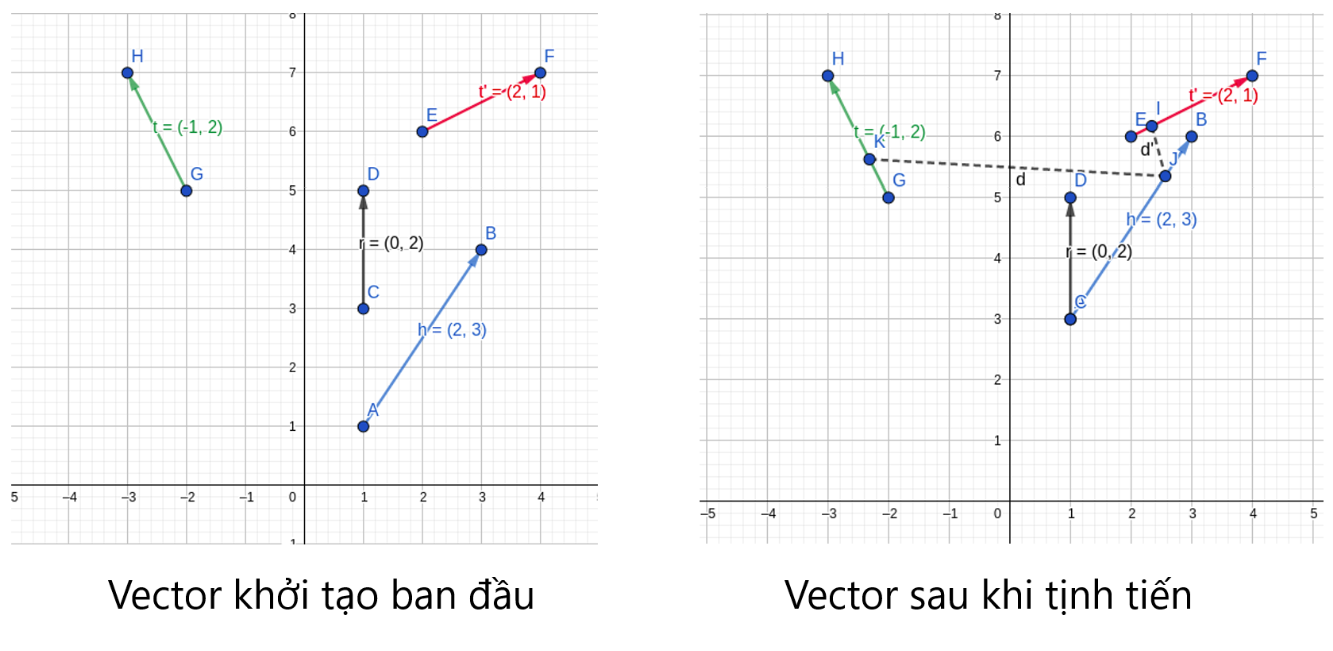
\includegraphics{images/transe.png}
	}
	\caption{TransE embedding model}
	\label{fig:TransEExplain}
\end{figure}

Here, $\gamma > 0$ is the margin, and $h'$ and $t'$ are entities sampled as defined in Equation \ref{eq:sampleTransE}. $\Delta$ and $\Delta'$ represent the difference vectors for the embeddings in valid and invalid triples, respectively, with $d = \big\|\Delta \big\|_{1} = \big\| \overrightarrow{h} + \overrightarrow{r} - \overrightarrow{t} \big\|_{1}$ and $d' = \big\|\Delta' \big\|_{1} = \big\| \overrightarrow{h'} + \overrightarrow{r} - \overrightarrow{t'} \big\|_{1}$, where $\|\cdot\|_{1}$ denotes the L1 norm.

As illustrated in \autoref{fig:TransEExplain}, if $d > d'$ or $d - d' > 0$, then $\overrightarrow{h} + \overrightarrow{r}$ is closer to $\overrightarrow{t}$ than to $\overrightarrow{t'}$. Since we want the embedding vectors to satisfy the condition in Equation \ref{eq:conditionTransE}, $\overrightarrow{h} + \overrightarrow{r}$ should be as close as possible to $\overrightarrow{t}$. That means, the closer $\overrightarrow{h} + \overrightarrow{r}$ is to $\overrightarrow{t'}$, the more incorrect it becomes.

Therefore, during training, we aim for $\Delta'$ to be as large as possible relative to $\Delta$. If $\Delta' > \Delta$ or $d' - d > 0$, there is no need to update the embedding weights further. Hence, in the loss function \ref{eq:KBGATLoss}, the term $[d - d' + \gamma]_{+}$ captures only the positive part because the negative part already satisfies the correctness of the condition in Equation \ref{eq:conditionTransE} during training.



\subsection{Encoder Model}
\label{sec:encodeKBGAT}

After obtaining the embedding vectors that capture spatial features of the knowledge graph, these embeddings are passed through the next embedding layer to further aggregate the neighborhood information of each entity.


\begin{figure}[htp]
	\centering
	\resizebox{\textwidth}{!}{%
		\begin{tikzpicture}[
			emb/.style={draw, circle,minimum width=.1em, thin, anchor=center},
			entityInit/.style={emb, fill=amber},
			relationInit/.style={emb, fill=azure},
			entityEmb/.style={emb, fill=gray},
			relationEmb/.style={emb, fill=deepcarminepink},
			entityPretrain/.style={emb, fill=deepmagenta},
			entityOut/.style={emb, fill=deepskyblue},
			box/.style={draw,rectangle, fill=none},
			embBox/.style={box ,rounded corners=0.2em, minimum width=1.3em},
			layerBox/.style={color=azure!80, box ,very thick,rounded corners=0.2em, minimum width=1.3em},
			textbox/.style={box,rounded corners=0.3em, fill=none, align=center, execute at begin node=\setlength{\baselineskip}{1em}},
			arrowStrong/.style={thick,->,>=stealth},
			arrowDash/.style={thick, ->,>=stealth, dash pattern=on 1.5mm off 0.7mm, postaction={decorate}},
			row/.style={draw, rectangle, font=\fontsize{0.6em}{1}\sffamily, align=center, text width=3.9em},
			arrowStyle/.style={-latex', font=\sffamily},
			mydot/.style={draw, circle, minimum size=0.1em, scale=0.2},
			]
			% 5
			% Root
			\draw node[textbox][text width=5.7em] (graphAttention2) {\small Graph Attention Layer $2_{\ref{eq:graphAttention2}}$};
			
			\draw node[textbox][minimum width=9.5em, minimum height=21em, left=1.5em of graphAttention2] (layer3) {};
			
			\draw node[embBox][minimum height=20.3em, left=2em of graphAttention2] (box10) {};
			\begin{scope}[every node/.style={below=0mm of box10.center}]
				\foreach \x in {1,...,12}
				{\draw node[entityEmb][yshift=(\x-4)*1.1em+0.55em] (ex10\x) {};}
				
				\foreach \x in {1,...,6}
				{\draw node[relationEmb](ey10\x)[yshift=-(\x+3)*1.1em+0.55em]{};}
			\end{scope}
			
			\draw node[embBox][minimum height=7em, left=2em of box10, yshift=5em] (box7) {};
			\draw node[embBox][minimum height=7em, left=2em of box10, yshift=-5em] (box9) {};
			\begin{scope}
				\foreach \x in {1,...,6}
				{\draw node[entityEmb](e7\x)[yshift=(\x-3)*1.1em, below=0mm of box7.center]{};}
				
				\foreach \x in {1,...,6}
				{\draw node[relationEmb](e9\x)[yshift=(\x-3)*1.1em, below=0mm of box9.center]{};}
			\end{scope}
			
			\draw node[embBox][minimum height=4em, left=2em of box7, yshift=2.5em] (box5) {};
			\draw node[embBox][minimum height=4em, left=2em of box7, yshift=-2.5em] (box6) {};
			\draw node[embBox][minimum height=5em, left=2em of box9] (box8) {};
			\begin{scope}
				\foreach \x in {1,...,3}
				{\draw node[entityEmb](e5\x)[yshift=(\x-2)*1.1em+0.55em, below=0mm of box5.center]{};}
				
				\foreach \x in {1,...,3}
				{\draw node[entityEmb](e6\x)[yshift=-(\x-2)*1.1em+0.55em, below=0mm of box6.center]{};}
				
				\foreach \x in {1,...,4}
				{\draw node[relationInit](e8\x)[yshift=(\x-2)*1.1em, below=0mm of box8.center]{};}
			\end{scope}
			\draw node[layerBox][minimum height=8em,minimum width=5.5em, left=1.5em of box10, yshift=-5em] (fc1) {};
			
			% Left
			\begin{scope}[every node/.style={left=2em of layer3}]
				\draw node[textbox][yshift=5.5em, text width=4em] (attentionHead1) {\small Attention Head 1};
				\draw node[textbox][yshift=-5.5em, text width=4em] (attentionHead2) {\small Attention Head 2};
			\end{scope}
			\draw node[textbox][left=1.5em of layer3, text width=5.5em, minimum width=5.8em, minimum height=16em] (graphAttention1) {\small Graph Attention Layer $1_{\ref{eq:graphAttention1}}$ };
			
			\draw node[textbox][minimum width=12.3em, minimum height=21em, left=1.5em of graphAttention1] (layer1) {};
			% Layer 1
			\draw node[embBox][minimum height=10.5em, yshift=1em,right=3em of layer1.center, left=2em of graphAttention1] (box4) {};
			\begin{scope}
				\foreach \x in {1,...,6}
				{\draw node[entityInit](ex4\x)[yshift=(\x-2)*1.1em-0.4em, above=0em of box4.center]{};}
				
				\foreach \x in {1,...,3}
				{\draw node[relationInit](e4y\x)[yshift=-(\x)*1.1em-0.6em, below=0mm of box4.center]{};}
			\end{scope}
			
			% Start Initial
			\draw node[embBox][minimum height=4em, yshift=4.5em, left=2em of box4] (box1) {};
			\foreach \x in {1,...,3}
			{\draw node[entityInit](e1\x)[yshift=(\x-2)*1.1em+0.5em, below=0mm of box1.center]{};}
			
			\draw node[embBox][minimum height=4em, left=2em of box4] (box2) {};
			\foreach \x in {1,...,3}
			{\draw node[relationInit](e2\x)[yshift=(\x-2)*1.1em+0.5em, below=0mm of box2.center]{};}
			
			\draw node[embBox][minimum height=4em, yshift=-4.5em, left=2em of box4] (box3) {};
			\foreach \x in {1,...,3}
			{\draw node[entityInit](e3\x)[yshift=(\x-2)*1.1em+0.5em, below=0mm of box3.center]{};}
			% Start Initial
			
			\begin{scope}[every node/.style={left=of box2, row}]
				\draw node (relation1) {president\_of};
				\draw node[above=0mm of relation1] (entity1) {Donald Trump};
				\draw node[above=0mm of entity1] (triple1) {Triple 1};
				\draw node[below=0mm of relation1] (entity2) {United States};	
			\end{scope}
			
			\begin{scope}[every node/.style={row}]
				\draw node[below=3em of entity2] (triple2) {Triple N};
				\draw node[below=0mm of triple2] (entity3) {Tom Cruise};
				\draw node[below=0mm of entity3] (relation2) {born\_in};
				\draw node[below=0mm of relation2] (entity4) {New York};	
			\end{scope}
			
			% Right
			\draw node[textbox][minimum height=16em, minimum width=2.3em, yshift=-4em, right=1.5em of graphAttention2] (layer4){};
			\draw node[embBox][minimum height=7em, right=2em of graphAttention2] (box11) {};
			\begin{scope}
				\foreach \x in {1,...,6}
				{\draw node[entityEmb](e11\x)[yshift=(\x-3)*1.1em, below=0mm of box11.center]{};}
			\end{scope}
			
			\draw node[embBox][minimum height=7em, below=0.7em of box11] (box12) {};
			\begin{scope}
				\foreach \x in {1,...,6}
				{\draw node[relationEmb](e12\x)[yshift=(\x-3)*1.1em, below=0mm of box12.center]{};}
			\end{scope}
			
			\draw node[embBox][minimum height=7em, above=1.5em of box11] (box13) {};
			\begin{scope}
				\foreach \x in {1,...,6}
				{\draw node[entityPretrain](e13\x)[yshift=(\x-3)*1.1em, below=0mm of box13.center]{};}
			\end{scope}
			
			\draw node[embBox][minimum height=5em, left=1.7em of box13] (box14) {};
			\begin{scope}
				\foreach \x in {1,...,4}
				{\draw node[entityInit](e14\x)[yshift=(\x-2)*1.1em, below=0mm of box14.center]{};}
			\end{scope}
			\draw node[layerBox][minimum height=8em, minimum width=5.5em, above=1.5em of box11, yshift=-0.5em, xshift=-1.5em] (fc2) {};
			
			\draw node[right=2em of box11, yshift=3.7em] (bigOTimes) {$\bigotimes^{\ref{eq:reInitEmbedding}}$};
			
			\draw node[textbox][minimum height=16em, minimum width=2.3em, yshift=-3.95em, right=1.5em of bigOTimes] (layer5) {};
			\draw node[embBox][minimum height=7em, above=1em of layer5.center, yshift=-0.5em] (box15) {};
			\begin{scope}
				\foreach \x in {1,...,6}
				{\draw node[entityOut](e15\x)[yshift=(\x-3)*1.1em, below=0mm of box15.center]{};}
			\end{scope}
			
			\draw node[embBox][minimum height=7em, below=1em of layer5.center, yshift=0.5em] (box16) {};
			\begin{scope}
				\foreach \x in {1,...,6}
				{\draw node[relationEmb](e16\x)[yshift=(\x-3)*1.1em, below=0mm of box16.center]{};}
			\end{scope}
			
			\draw node[textbox][right=1.5em of layer5] (final) {$\mathcal{L}_{\ref{eq:KBGATLoss}}$};
			%16
			% Arrow
			\draw [arrowStrong] (box10) -- (graphAttention2.west);
			
			\draw [arrowStrong] (entity1.east) -- (box1.west);
			\draw [arrowStrong] (relation1) -- (box2.west);
			\draw [arrowStrong] (entity2.east) -- (box3.west);
			
			\draw [arrowStrong] (graphAttention2.east) -- (box11.west);
			\draw [arrowStrong] (graphAttention2.east) -- (box12.west);
			
			\draw [arrowStrong] (box11.east) to ([xshift=0.35em] bigOTimes.west);
			\draw [arrowStrong] (box13.east) to ([xshift=0.35em] bigOTimes.west);
			
			\draw [arrowStrong] ([xshift=-1.7em] bigOTimes.east) -- (box15.west);
			
			\draw [arrowStrong] (box16.east) -- (final.west);
			\draw [arrowStrong] (box15.east) -- (final.west);
			
			\foreach \x in {1,2}
			\draw [arrowStrong] (layer1.east) -- (attentionHead\x.west);
			
			\foreach \x in {1,2}
			\draw [arrowStrong] (attentionHead\x.east) -- (layer3.west);
			
			\foreach \x in {1,2,3}
			\draw [arrowDash] (box\x.east) -- (box4.west);
			
			\foreach \x in {7,9}
			{\draw [arrowDash] (box\x) -- (box10.west);}
			
			\foreach \x in {5,6}
			{\draw [arrowDash] (box\x) -- (box7.west);}
			
			\foreach \x in {1, ..., 6}
			{\draw [thick] (e81) -- (e9\x);}
			\foreach \x in {1, ..., 6}
			{\draw [thick] (e82) -- (e9\x);}
			\foreach \x in {1, ..., 6}
			{\draw [thick] (e83) -- (e9\x);}
			\foreach \x in {1, ..., 6}
			{\draw [thick] (e84) -- (e9\x);}
			
			\foreach \x in {1, ..., 6}
			{\draw [thick] (e141) -- (e13\x);}
			\foreach \x in {1, ..., 6}
			{\draw [thick] (e142) -- (e13\x);}
			\foreach \x in {1, ..., 6}
			{\draw [thick] (e143) -- (e13\x);}
			\foreach \x in {1, ..., 6}
			{\draw [thick] (e144) -- (e13\x);}
			
			\draw node[mydot][below=1.1em of entity2] (dot1) {};
			\draw node[mydot][below=1.4em of entity2] (dot2) {};
			\draw node[mydot][below=1.7em of entity2] (dot3) {};
		\end{tikzpicture}
	}
	\caption{Illustration of the encoder layers in the KBGAT model}
	\label{fig:encoderKBGAT}
\end{figure}


The model transforms the entity embedding matrix

\[
\mathbf{E} = \Big\{\overrightarrow{e_1}, \overrightarrow{e_2}, ...,  \overrightarrow{e_{N_e}}\Big\} \xrightarrow{} \mathbf{E''} = \Big\{\overrightarrow{e''_1}, \overrightarrow{e''_2}, ...,  \overrightarrow{e''_{N_e}}\Big\},
\]
with $\mathbf{E} \in \mathbb{R}^{N_e \times D_{\text{in}}}$ and $\mathbf{E''} \in \mathbb{R}^{N_e \times D''}$.

Simultaneously, it transforms the relation embedding matrix

\[
\mathbf{R} = \Big\{\overrightarrow{r_1}, \overrightarrow{r_2}, ...,  \overrightarrow{r_{N_r}}\Big\} \xrightarrow{} \mathbf{R''} = \Big\{\overrightarrow{r''_1}, \overrightarrow{r''_2}, ...,  \overrightarrow{r''_{N_r}}\Big\},
\]
with $\mathbf{R} \in \mathbb{R}^{N_r \times P_{\text{in}}}$ and $\mathbf{R''} \in \mathbb{R}^{N_r \times P''}$.

Similar to the GAT model described in Section~\ref{sec:GAT}, the model transforms the entity embedding vectors from $D_{\text{in}}$ dimensions to $D''$ dimensions by aggregating neighborhood information through attention coefficients. $P_{\text{in}}$ and $P''$ are the input and output dimensions of the relation embedding vectors, respectively. $N_e$ and $N_r$ are the sizes of the entity and relation sets in $\mathcal{G}_{know}$, respectively.

The KBGAT model concatenates the entity and relation embedding vectors according to the following structure:

\begin{equation}
	\label{attentionWithRelation}
	\overrightarrow{t_{ijk}} = \mathbf{W_1} [\overrightarrow{e_i} || \overrightarrow{e_j} || \overrightarrow{r_k}]
\end{equation}

Here, $\overrightarrow{t_{ijk}}$ is the embedding vector representing the triple $t_{ij}^k = (e_i, r_k, e_j)$, where $e_j$ and $r_k$ are the neighboring entity and the relation connecting the source node $e_i$ to the node $e_j$. $\mathbf{W_1} \in \mathbb{R}^{D_k \times (2 D_{\text{in}} + P_{\text{in}})}$ is a weight matrix that performs a linear transformation of the concatenated input vectors into a new vector with dimensionality $D_k$. These weight matrices are either randomly initialized using a normal distribution or pre-trained using the TransE model~\cite{bordes2013translating}.

Similar to Equation~\ref{attentionCoeff} in the GAT model, we need to compute the attention coefficient for each edge with respect to a given node. Then, the \textit{softmax} function is applied to normalize these coefficients as follows:

\begin{equation}
	\label{attentionRelationCoeff}
	\begin{split}
		\alpha_{ijk}& = \text{softmax}_{jk}(\text{LeakyReLU}(\mathbf{W_2} \overrightarrow{t_{ijk}}))\\
		&= \frac{
			\text{exp} \Big( \text{LeakyReLU} \Big( \mathbf{W_2} \overrightarrow{t_{ijk}}\Big) \Big)
		}
		{
			\sum_{n\in \mathcal{N}_i} \sum_{r\in \mathcal{R}_{in}}
			\text{exp} \Big( \text{LeakyReLU} \Big( \mathbf{W_2} \overrightarrow{t_{inr}} \Big) \Big)
		}
	\end{split}
\end{equation}


%Trong đồ thị, mỗi cạnh của thực thể không chỉ được biểu diễn thông tin bởi thực thể đầu $e_\text{head}$ và thực thể đích $e_\text{tail}$ mà có các quan hệ giữa chúng. Hơn nữa trong một cạnh, các thực thể còn có thể đóng nhiều vai trò khác nhau phụ thuộc vào các loại quan hệ khác nhau. Vì vậy phương pháp KBGAT bổ sung thêm thông tin của một vector nhúng quan hệ vào một cạnh  nhúng $(\overrightarrow{e_\text{i}}, \overrightarrow{r_k}, \overrightarrow{e_\text{j}})$. Tuy nhiên một vector $\overrightarrow{e_i}$ hay $\overrightarrow{r_k}$ không thể biểu thị một cách đầy đủ tri thức của một thực thể $e_i$ hay quan hệ $r_k$ trong một đồ thị, vì một tri thức sẽ có thể có mối liên hệ với những tri thức lân cận hay nói cách khác một \textbf{thực thể nhúng} (entity embedding) hay một \textbf{quan hệ nhúng} (relation embedding) sẽ cần thêm thông tin của các vector nhúng của thực thể lân cận và quan hệ lân cận khác để có thể là một đại diện đầy đủ . Chính vì vậy phương pháp \textit{n-hop neighborhood} \cite{lin2018multi} sẽ giúp bổ sung thêm thông tin lân cận của thực thể $e_i$ và quan hệ $r_k$ bằng cách ghép chồng để tạo thành một vector mới theo công thức sau :
%\begin{align}
%{\overrightarrow{h_i} = [\overrightarrow{e_i} \bigparallel_{\text{axis}=1} \overrightarrow{e_{i_{\text{n-hop}}}}]} \hspace{0.5cm};\hspace{1.5cm}&
%{\overrightarrow{g_k} = [\overrightarrow{r_k} \bigparallel_{\text{axis}=1} \overrightarrow{r_{k_{\text{n-hop}}}}]}
%\end{align}
%
%Trong đó $\overrightarrow{h_i}$, $\overrightarrow{g_k}$ tương ứng là vector nhúng mới của thực thể $e_i$ và các thực thể lân cận ($e_{i_{\text{n-hop}}}$) hay quan hệ $r_k$ và các quan hệ lân cận ($r_{k_{\text{n-hop}}}$); ký hiệu $\bigparallel_{\text{axis}=1}$ biểu thị cho phép xếp chồng lên nhau. Các vector $\overrightarrow{e_{i_{\text{n-hop}}}}$ và $\overrightarrow{r_{k_{\text{n-hop}}}}$ được tính bằng tổng vector nhúng của các thực thể hoặc các quan hệ lân cận đi qua $n-hop$ độ sâu bắt đầu từ $e_i$ theo công thức sau : 
%
%\begin{align}
%{\overrightarrow{e_{i_{\text{n-hop}}}} = \bigparallel_{d=1}^{\text{n-hop}} \sum_{n \in \mathcal{N}_i} \overrightarrow{e_n^d}} \hspace{0.5cm};\hspace{1.5cm}&
%{\overrightarrow{r_{k_{\text{n-hop}}}} = \bigparallel_{d=1}^{\text{n-hop}} \sum_{m \in \mathcal{N}_k} \overrightarrow{r_m^d}}
%\end{align}
%
%Với mối thực thể $e_n$ hay quan hệ $r_m$ có độ sâu d (depth) bắt đầu từ thực thể $e_i$, ta sẽ tính tổng các vector nhúng và ghép chồng với nhau.
%
%Để biểu thị cho quá trình biến tuyến tính của vector nhúng, ta cho mỗi vector nhúng đi qua một ma trận trọng số : $\overrightarrow{h'_i} = \mathbf{W}_{\text{entity}} \overrightarrow{h_i}$ 
%và $\overrightarrow{g'_i} = \mathbf{W}_{\text{relation}} \overrightarrow{g_i}$. Tuy nhiên để thu được một trọng số mới biểu diễn bộ ba $t^k_{ij} = (e_{\text{head}}, relation, e_{\text{tail}})$ tương ứng với một cạnh trong trong KB. Ta thực hiện quá trình biến đổi tuyến tính đó bằng cách ghép cả thực thể và mối quan hệ với nhau rồi nhân với một ma trận trọng số chung như công thức sau :
%
%trong đó $\overrightarrow{t_{ijk}}$ là một vector nhúng biểu diễn cho một bộ ba $t^k_{ij}$. Các vector $\overrightarrow{h_i}$, $\overrightarrow{h_j}$ và $\overrightarrow{g_j}$ tương ứng là vector nhúng của các thực thể $e_i$, $e_j$ và quan hệ $r_k$. $\mathbf{W_1} \in \mathbb{R}^{3 T \times S^\text{batch}}$ . Để áp dụng cơ chế chú ý (attention mechanisms \cite{vaswani2017attention}), ta cần học sự quan trọng của một cạnh $t_{ij}^k$ bởi giá trị của $b_{ij}^k$. Để tham số hóa quá trình biến đổi tuyến tính ta nhân với ma trận trọng số $\mathbb{W}_{2}$ và lấy giá trị chú ý tuyệt đối bằng hàm $LeakyRelu$ theo công thức sau :
%
%\begin{align}
%b_{ijk} = \text{LeakyRelu}\Big( \mathbf{W_2} t_{ijk} \Big)
%\end{align}
%
%Sau đó, với mỗi độ lớn của $b^k_{ij}$ được cho qua hàm \textit{softmax} để tính giá trị thể hiện xác suất của từng giá trị chú ý $\alpha_{ijk}$ đối với từng bộ ba .
where $\mathcal{N}_i$ denotes the set of neighbors of the central node $e_i$ within $n_{\text{hop}}$ hops; $\mathcal{R}_{in}$ represents the set of all relations that exist along the paths connecting the source entity $e_i$ to a neighboring entity $e_n \in \mathcal{N}_i$. Similar to Equation~\ref{scaleAttentionCoef}, the embedding vectors $\overrightarrow{t^k_{ij}}$ are scaled by their corresponding normalized attention coefficients:

\begin{align}
	{\overrightarrow{e'_{i}}}&={\sigma\left(\sum_{j \in \mathcal{N}_i} \sum_{k \in \mathcal{R}_{ij}} \alpha_{ijk} \overrightarrow{t_{ijk}}\right)}
\end{align}

Similar to the multi-head attention mechanism in Equation~\ref{multiHeadAttention}, we concatenate $N_{\text{head}}$ attention heads to stabilize the learning process:

\begin{equation}
	\label{eq:graphAttention1}
	\overrightarrow{e'}_i=\bigparallel_{h=1}^{N_{\text{head}}} \sigma\left(\sum_{j\in \mathcal{N}_i}\alpha_{ijk}^{(h)} \overrightarrow{t^{(h)}_{ijk}}\right)
\end{equation}

Likewise, for relation embeddings, a weight matrix $\mathbf{W}_R$ is used to perform a linear transformation from the original relation embedding of dimension $P$ to a new dimension $P'$:

\begin{align}
	\mathbf{R'} = \mathbf{R} \mathbf{W}^R; \hspace{2cm} \text{where: } \mathbf{W}^R \in \mathbb{R}^{P \times P'}
\end{align}





At this stage, we have obtained two matrices: $\mathbf{H}' \in \mathbb{R}^{N_e \times D'}$ and $\mathbf{R}' \in \mathbb{R}^{N_r \times P'}$, which are the updated entity and relation embedding matrices, respectively, with new dimensions. The model proceeds through the final attention layer, taking as input the newly updated entity and relation embeddings as shown in Equation~\ref{multiHeadConcat}. However, if we apply multi-head attention at this final layer for prediction, the concatenation operation will no longer be \textit{sensitive} to the self-attention mechanism. Therefore, instead of concatenating, the model averages the outputs and then applies a final non-linear activation function:

\begin{equation}
	\label{eq:graphAttention2}
	\overrightarrow{e''_{i}}=\sigma\left(\frac{1}{N_{\text{head}}} \sum_{h=1}^{N_{\text{head}}} \sum_{j \in \mathcal{N}_i} \sum_{k \in \mathcal{R}_{ij}} \alpha'^{(h)}_{ijk} \overrightarrow{t'^{(h)}_{ijk}} \right)
\end{equation}

where $\alpha'^{(h)}_{ijk}$ and $t'^{(h)}_{ijk}$ denote the normalized attention coefficients and the triple embedding vectors for $(e_i, r_k, e_j)$ in attention head $(h)$, respectively.

Up to this point, the KBGAT model functions similarly to the GAT model in Section~\ref{sec:GAT}, but it additionally incorporates both entity embedding information and neighbor nodes up to $n_{\text{hop}}$ hops. This results in the final entity embedding matrix $\mathbf{E}'' \in \mathbb{R}^{N_e \times D''}$ and the final relation embedding matrix $\mathbf{R}'' \in \mathbb{R}^{N_r \times P''}$. 

However, after the embedding learning process, the final entity embedding matrix $\mathbf{E}''$ may lose the initial embedding information due to the \textbf{vanishing gradient} problem. To address this, the model employs residual learning, by projecting the initial embedding matrix $\mathbf{E}$ through a weight matrix $\mathbf{W}^E \in \mathbb{R}^{D_{\text{in}} \times D''}$, and then directly adding it to the final embedding, thus preserving the initial embedding information during training:

\begin{equation}
	\label{eq:reInitEmbedding}
	\mathbf{H} = \mathbf{W}^E \mathbf{E} + \mathbf{E''}
\end{equation}

Finally, the training datasets are sampled to generate valid triples and invalid triples, similar to the TransE model described above, in order to learn the embedding vectors. However, the distance between embedding vectors is computed using the L1 norm as follows:
\[
d_{t_{ij}} = \big|\big|\vec{h_i}+ \vec{g_k}-\vec{h_j}\big|\big|_1
\]

Similarly, we train the model using a margin-based loss function:

\begin{equation}
	L(\Omega)=\sum_{t_{ij} \in S} \sum_{t'_{ij} \in S'} \text{max}\{d_{t'_{ij}} - d_{t_{ij}} + \gamma , 0 \}
\end{equation}

where $\gamma > 0$ is the margin parameter, $S$ is the set of valid triples, and $S'$ is the set of invalid triples, defined as:

\begin{equation}
	{S'} ={\underbrace{\{ t^k_{i'j} | e'_i \in \mathcal{E}\setminus e_i\}}_{\text{head entity replacement}} \cup \underbrace{\{ t^k_{ij'} | e'_j \in \mathcal{E}\setminus e_j\}}_{\text{tail entity replacement}}}
\end{equation}

The output of the KBGAT model is the set of entity and relation embedding vectors, which are subsequently fed into the ConvKB model for final prediction.




\subsection{ConvKB Prediction Model}
\label{sec:predictionConvKB}

\begin{figure}[htp]
	\centering
	\resizebox{\textwidth}{!}{%
		\begin{tikzpicture}[
			emb/.style={draw, circle,minimum width=.1em, thin, anchor=center},
			head/.style={emb, fill=amber},
			relation/.style={emb, fill=azure},
			tail/.style={emb, fill=awesome},
			conv/.style={emb, fill=gray},
			box/.style={draw,rectangle, fill=none},
			embBox/.style={box ,rounded corners=0.2em},
			convBox/.style={box, minimum height=1.3em, minimum width=4.8em,rounded corners=0.2em},
			convolution/.style={box, minimum height=1.3em, minimum width=4.5em,rounded corners=0.2em},
			convLayer/.style={box, minimum height=1.05em, minimum width=5em, rounded corners=0.2em},
			textbox/.style={box,rounded corners=0.3em, fill=none, align=center},
			title/.style={fill=none, align=center},
			arrow/.style={thick,>=stealth},
			arrowStrong/.style={thick,->,>=stealth},
			arrowStyle/.style={-latex'},
			mydot/.style={draw, circle, minimum size=0.1em, scale=0.2},
			]
			% 5
			%			\draw node[textbox] (lossConvKB) {$\mathcal{L}\ref{eq:lossConvKB}$};
			\draw node[textbox] (lossConvKB) {score};
			
			\draw node[embBox][minimum width=1.3em, minimum height=14em, left=2em of lossConvKB] (box9) {};
			\foreach \x in {1,...,4}
			{\draw node[head](e9\x)[yshift=-(\x-7)*1.1em, below=0mm of box9.center]{};}
			
			\foreach \x in {1,...,4}
			{\draw node[relation](e8\x)[yshift=(\x-2)*1.1em, below=0mm of box9.center]{};}
			
			\foreach \x in {1,...,4}
			{\draw node[tail](e7\x)[yshift=(\x-6)*1.1em, below=0mm of box9.center]{};}
			
			%
			\draw node[convBox][yshift=3.8em, left=2em of box9] (box6) {};
			\foreach \x in {1,...,4}
			{\draw node[head](e6\x)[yshift=0.5em, xshift=(\x-2)*1.1em-0.5em, below=0mm of box6.center]{};}
			
			\draw node[convBox][left=2em of box9] (box5) {};
			\foreach \x in {1,...,4}
			{\draw node[relation](e5\x)[yshift=0.5em, xshift=(\x-2)*1.1em-0.5em, below=0mm of box5.center]{};}
			
			\draw node[convBox][yshift=-3.8em, left=2em of box9] (box4) {};
			\foreach \x in {1,...,4}
			{\draw node[tail](e4\x)[yshift=0.5em, xshift=(\x-2)*1.1em-0.5em, below=0mm of box4.center]{};}
			
			%
			\draw node[convolution][left=2em of box5] (filterBox1) {};
			\foreach \x in {1,...,3}
			{\draw node[conv, fill=amber](filter1\x)[yshift=0.5em, xshift=(\x-2)*1.1em, below=0mm of filterBox1.center]{};}
			\foreach \x in {1,...,3}
			{\draw node[conv, fill=azure](filter2\x)[yshift=0.5em, xshift=(\x-2)*1.1em+0.2em, below=0mm of filterBox1.center]{};}
			\foreach \x in {1,...,3}
			{\draw node[conv, fill=awesome](filter3\x)[yshift=0.5em, xshift=(\x-2)*1.1em+0.4em, below=0mm of filterBox1.center]{};}
			
			\draw node[embBox][minimum width=1.3em, minimum height=5em, xshift=-1.5em, left=4em of filterBox1] (box1) {};
			\foreach \x in {1,...,4}
			{\draw node[head, fill=amber!30](e1\x)[yshift=(\x-2)*1.1em, below=0mm of box1.center]{};}
			\draw node[title][above=0mm of box1] (headText) {\small $\text{h}$};
			
			\draw node[embBox][minimum width=1.3em, minimum height=5em, left=4em of filterBox1] (box2) {};
			\foreach \x in {1,...,4}
			{\draw node[relation, fill=azure!30](e2\x)[yshift=(\x-2)*1.1em, below=0mm of box2.center]{};}
			\draw node[title][above=0mm of box2] (relationText) {\small $\text{r}$};
			
			\draw node[embBox][minimum width=1.3em, minimum height=5em, xshift=1.5em,left=4em of filterBox1] (box3) {};
			\draw node[title][above=0mm of filterBox1] (filterTitle) {\small $3.\omega^{\text{1} \times \text{3}}$};
			\foreach \x in {1,...,4}
			{\draw node[tail, fill=awesome!30](e3\x)[yshift=(\x-2)*1.1em, below=0mm of box3.center]{};}
			\draw node[title][above=0mm of box3] (tailText) {\small $\text{t}$};
			
			\draw node[convLayer, color=red][yshift=1.71em, left=2em of filterBox1] (conv1){};
			\draw node[convLayer, color=green][yshift=0.61em, left=2em of filterBox1] (conv2){};
			\draw node[convLayer, color=blue][yshift=-0.5em, left=2em of filterBox1] (conv3){};
			\draw node[convLayer, color=amber][yshift=-1.6em, left=2em of filterBox1] (conv4){};
			
			% Arrow
			\foreach \x in {1,...,4}
			\draw [arrowStrong] (conv\x.east) -- (filterBox1.west);
			
			\foreach \x in {4,...,6}
			\draw [arrowStrong] (filterBox1.east) -- (box\x.west);
			
			\draw [arrow] (box4.east) -- (box9.south west);
			\draw [arrow] (box5.east) -- (box9.west);
			\draw [arrow] (box6.east) -- (box9.north west);
			
			\foreach \x in {1,...,4}
			\draw [arrow] (e9\x.east) -- (lossConvKB.west);
			\foreach \x in {1,...,4}
			\draw [arrow] (e8\x.east) -- (lossConvKB.west);
			\foreach \x in {1,...,4}
			\draw [arrow] (e7\x.east) -- (lossConvKB.west);
			
		\end{tikzpicture}
	}
	\caption{Illustration of the decoder layers of the ConvKB model with 3 filters}
	\label{fig:decoderConvKB}
\end{figure}


After mapping entities and relations into a low-dimensional space, the model employs ConvKB \cite{nguyen2017novel} to analyze the global features of a triple $t_{ijk}$ across each dimension, thereby generalizing transformation patterns through convolutional layers. The scoring function with the learned feature mappings is defined as follows:

\begin{equation}
	f(t_{ijk}) = \Big( \bigparallel_{m=1}^{\Omega} \text{ReLU} ([\overrightarrow{e_i}, \overrightarrow{r_k}, \overrightarrow{h_j}] \ast \omega^m)\Big).\mathbf{W}
\end{equation}

where $\omega^m$ denotes the $m$-th convolutional filter,  
$\Omega$ is the hyperparameter representing the number of convolutional layers,  
$\ast$ denotes the convolution operation, and  
$\mathbf{W} \in \mathbb{R}^{\Omega k \times 1}$ is the linear transformation matrix used to compute the final score for the triple.  

The model is trained using a soft-margin loss function as follows:

\begin{equation}
	\label{eq:lossConvKB}
	\mathcal{L} = \sum_{t^k_{ij} \in \{S \cup S'\}} \text{log}(1 + \exp(l_{t^k_{ij}} \cdot f(t^k_{ij}))) + \frac{\lambda}{2} \parallel{\mathbf{W}}\parallel_2^2
\end{equation}

where 

\[
l_{t^k_{ij}} = 
\begin{cases}
	1 & \text{for } t^k_{ij} \in S \\
	-1 & \text{for } t^k_{ij} \in S' \\
\end{cases}
\]

The final output of the ConvKB model is the ranking score corresponding to each prediction.
